\chapter[L'application]{Présentation de l'application}

Dans ce chapitre on présente l'application Crazy Wolf. 
Au travers d'images commentées nous allons décrire les scénarios
d'utilisation les plus communs.
\section[Authentification \& écran d'accueil - Scénario I]{Scénario I}
\subsection*{Authentification \& écran d'accueil}
Ici la serveuse Kim, qui n'a pas de privilèges, c'est-à-dire qu'elle n'est 
ni manager ni administratrice, se connecte et accède au premier écran possible.
Puis elle, clic sur \textit{Mes services}.

\begin{figure}[!h]
    \centering
    \begin{subfigure}{.3\textwidth}
        \centering
        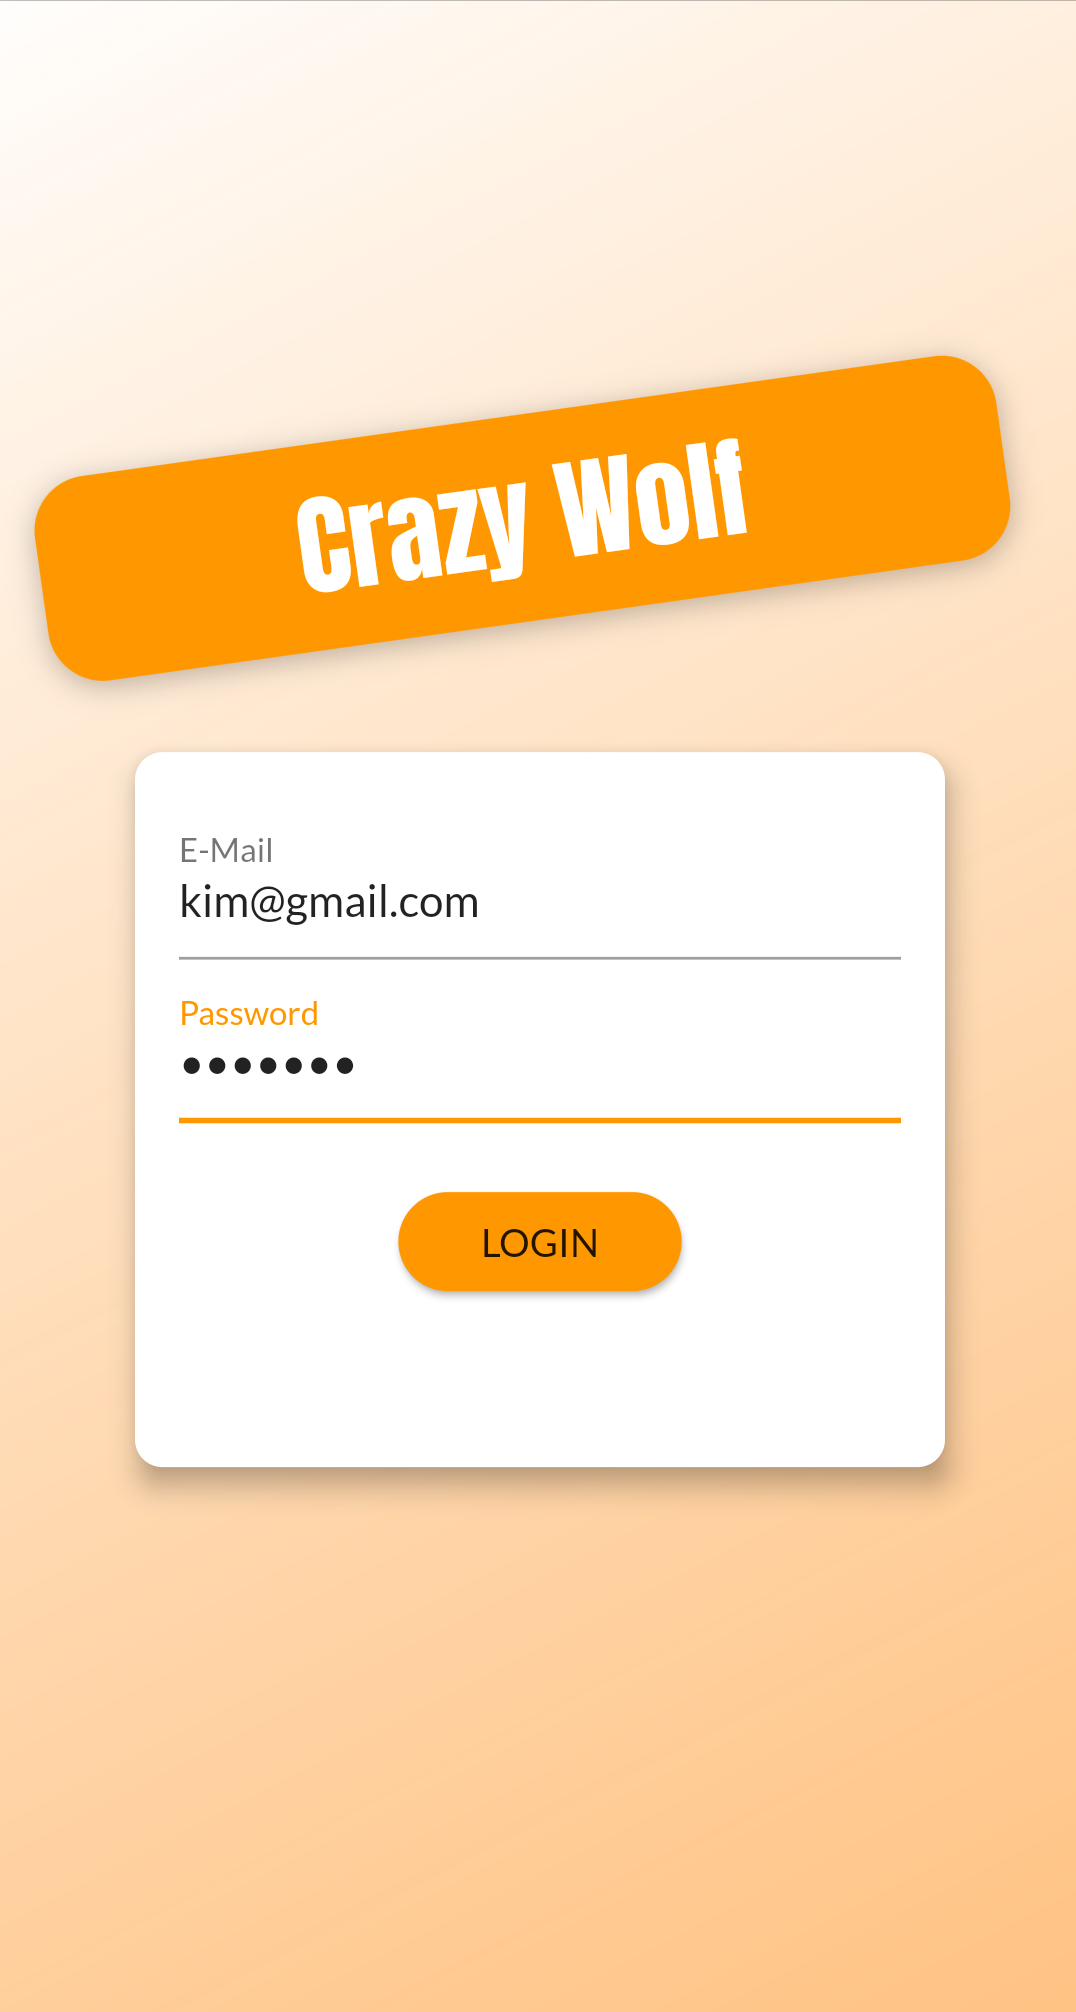
\includegraphics[width=0.9\linewidth]{screenshots/scenario_01/login.png}
        \caption{login}
        \label{fig:login}
    \end{subfigure}
    \begin{subfigure}{.3\textwidth}
        \centering
        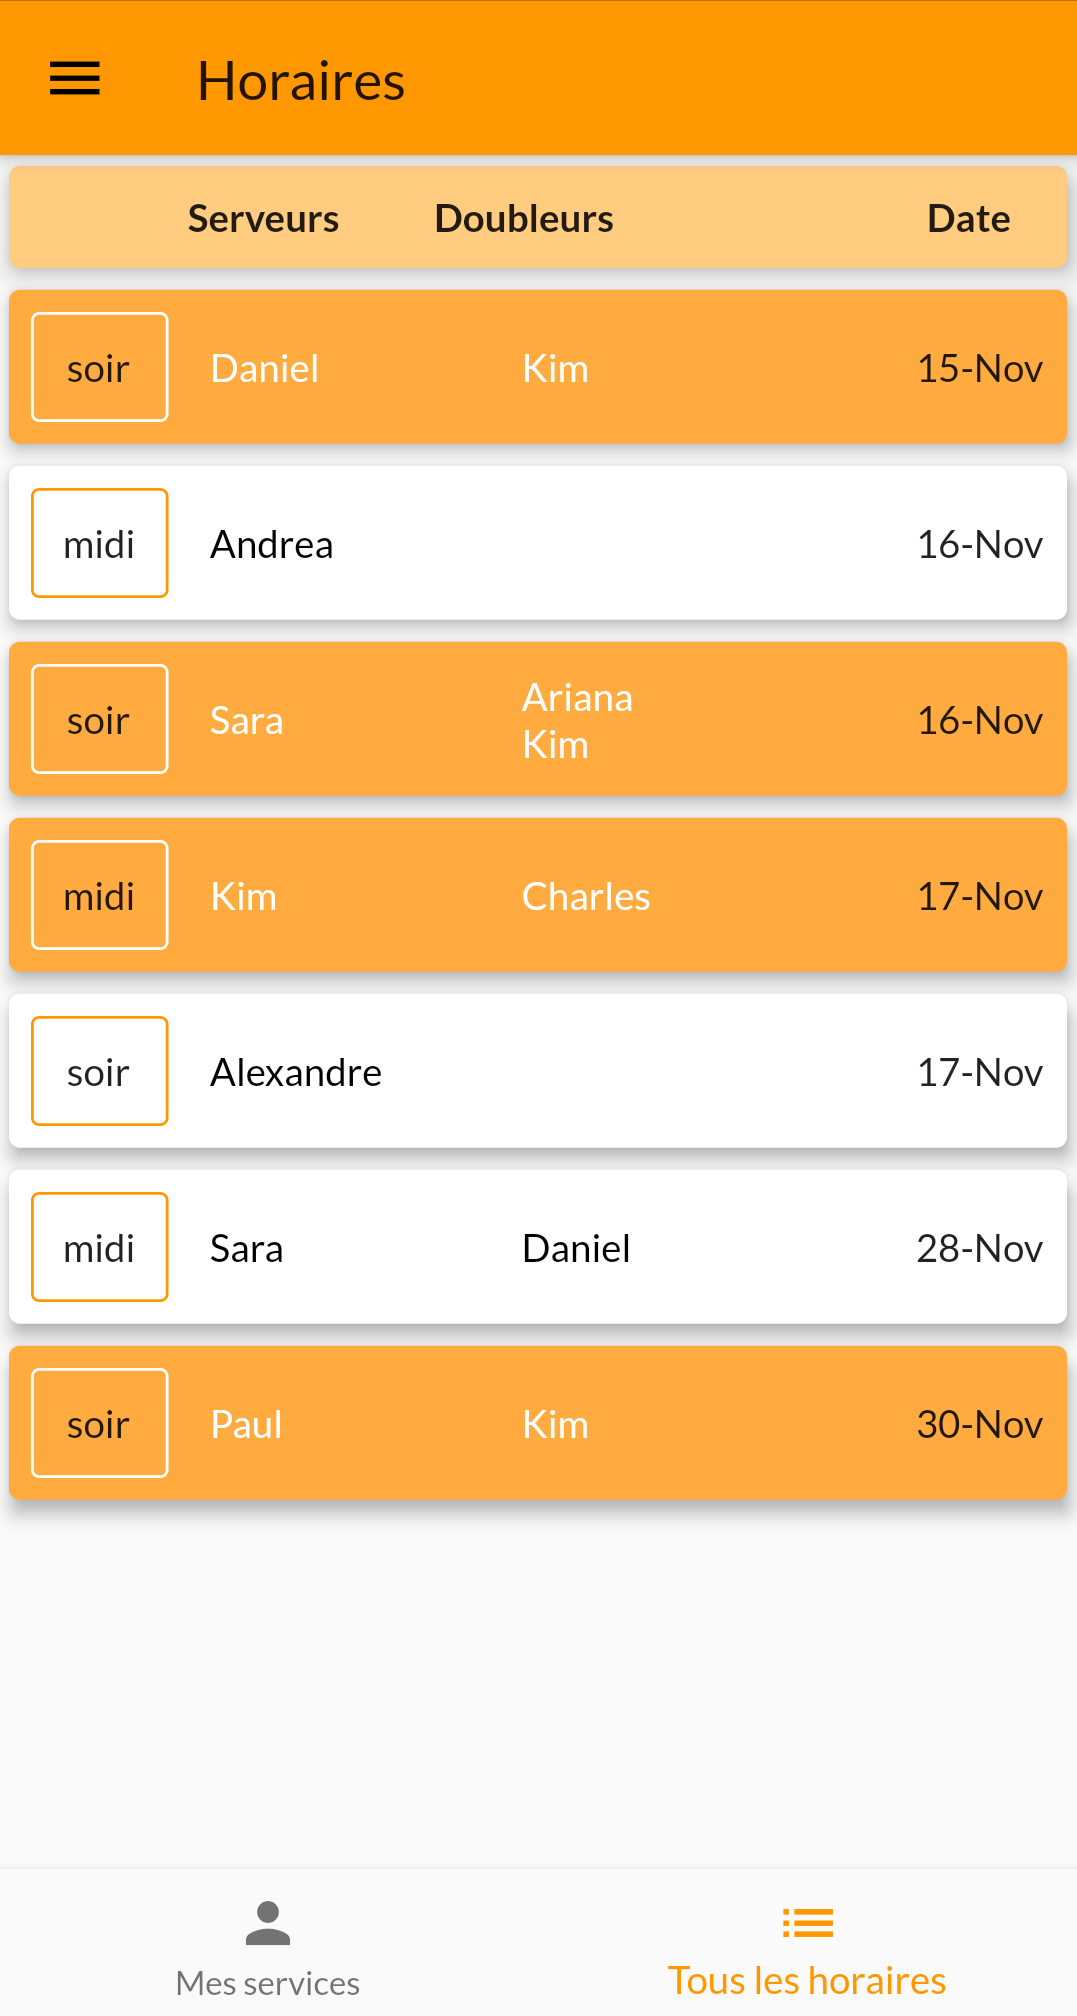
\includegraphics[width=0.9\linewidth]{screenshots/scenario_01/horaires.png}
        \caption{horaires}
        \label{fig:horaires}
    \end{subfigure}
    \begin{subfigure}{.3\textwidth}
        \centering
        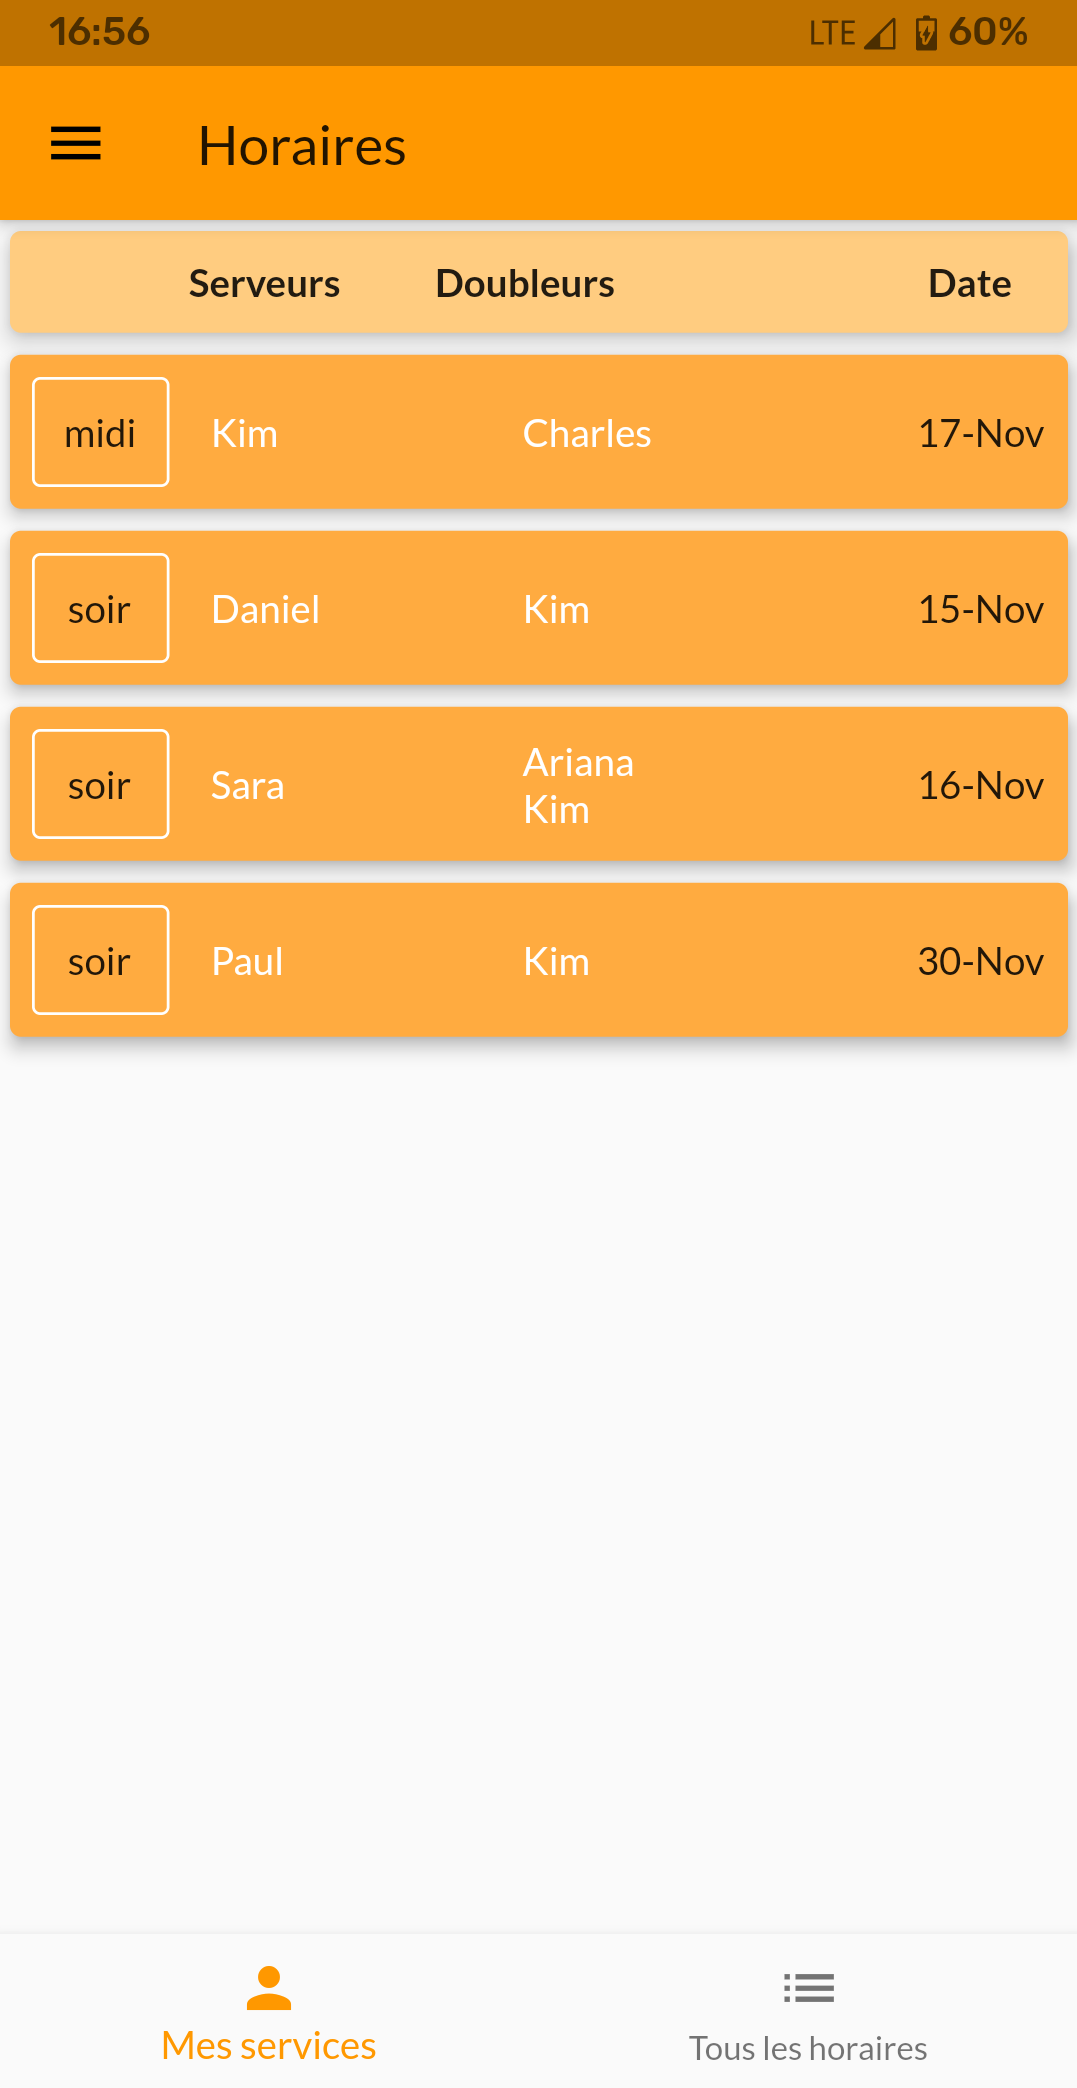
\includegraphics[width=0.9\linewidth]{screenshots/scenario_01/mesHoraires.png}
        \caption{mes horaires}
        \label{fig:mesHoraires}
    \end{subfigure}
    \caption{scénario I}
    \label{fig:scen01}
\end{figure}

L'utilisateur doit dans un premier temps se connecter à l'aide d'identifiants déjà existant dans l'écran \ref{fig:login}. Une fois l'adresse mail et le mot de passe saisis, 
l'écran \textit{Horaires} \ref{fig:horaires} s'affiche. 


On y voit l'ensemble des horaires de travail. Les services sont définis par
\begin{itemize}
    \item le type: midi ou soir.
    \item un ou plusieurs serveurs.
    \item zéro, un ou plusieurs doubleurs.
    \item la date
\end{itemize}
Les services sont ordonnés par date, les jours précédents au moment de la connexion ne 
sont pas affichés. Les horaires correspondant à la personne authentifié sont de couleurs orange.

Les services sont affichés sous forme de liste scrollable.

On peut également naviguer à l'aide du menu inférieur à \textit{Mes services} où seuls les horaires du serveur authentifié sont affichés. Comme on le voit 
dans \ref{fig:mesHoraires}

\section[Mise en bourse d'un service - Scénario II]{Scénario II}
    \subsection*{Mise en bourse d'un service}
    Supposons que Kim, la serveuse authentifiée ne puisse pas travailler le 17 novembre.
    Elle souhaite donc se faire remplacer. Pour se faire, dans l'onglet 
    \textit{Horaires}, elle peut mettre son service en bourse en glissant le 
    service en question sur la gauche.
    \begin{figure}[!h]
        \centering
        \begin{subfigure}{.3\textwidth}
            \centering
            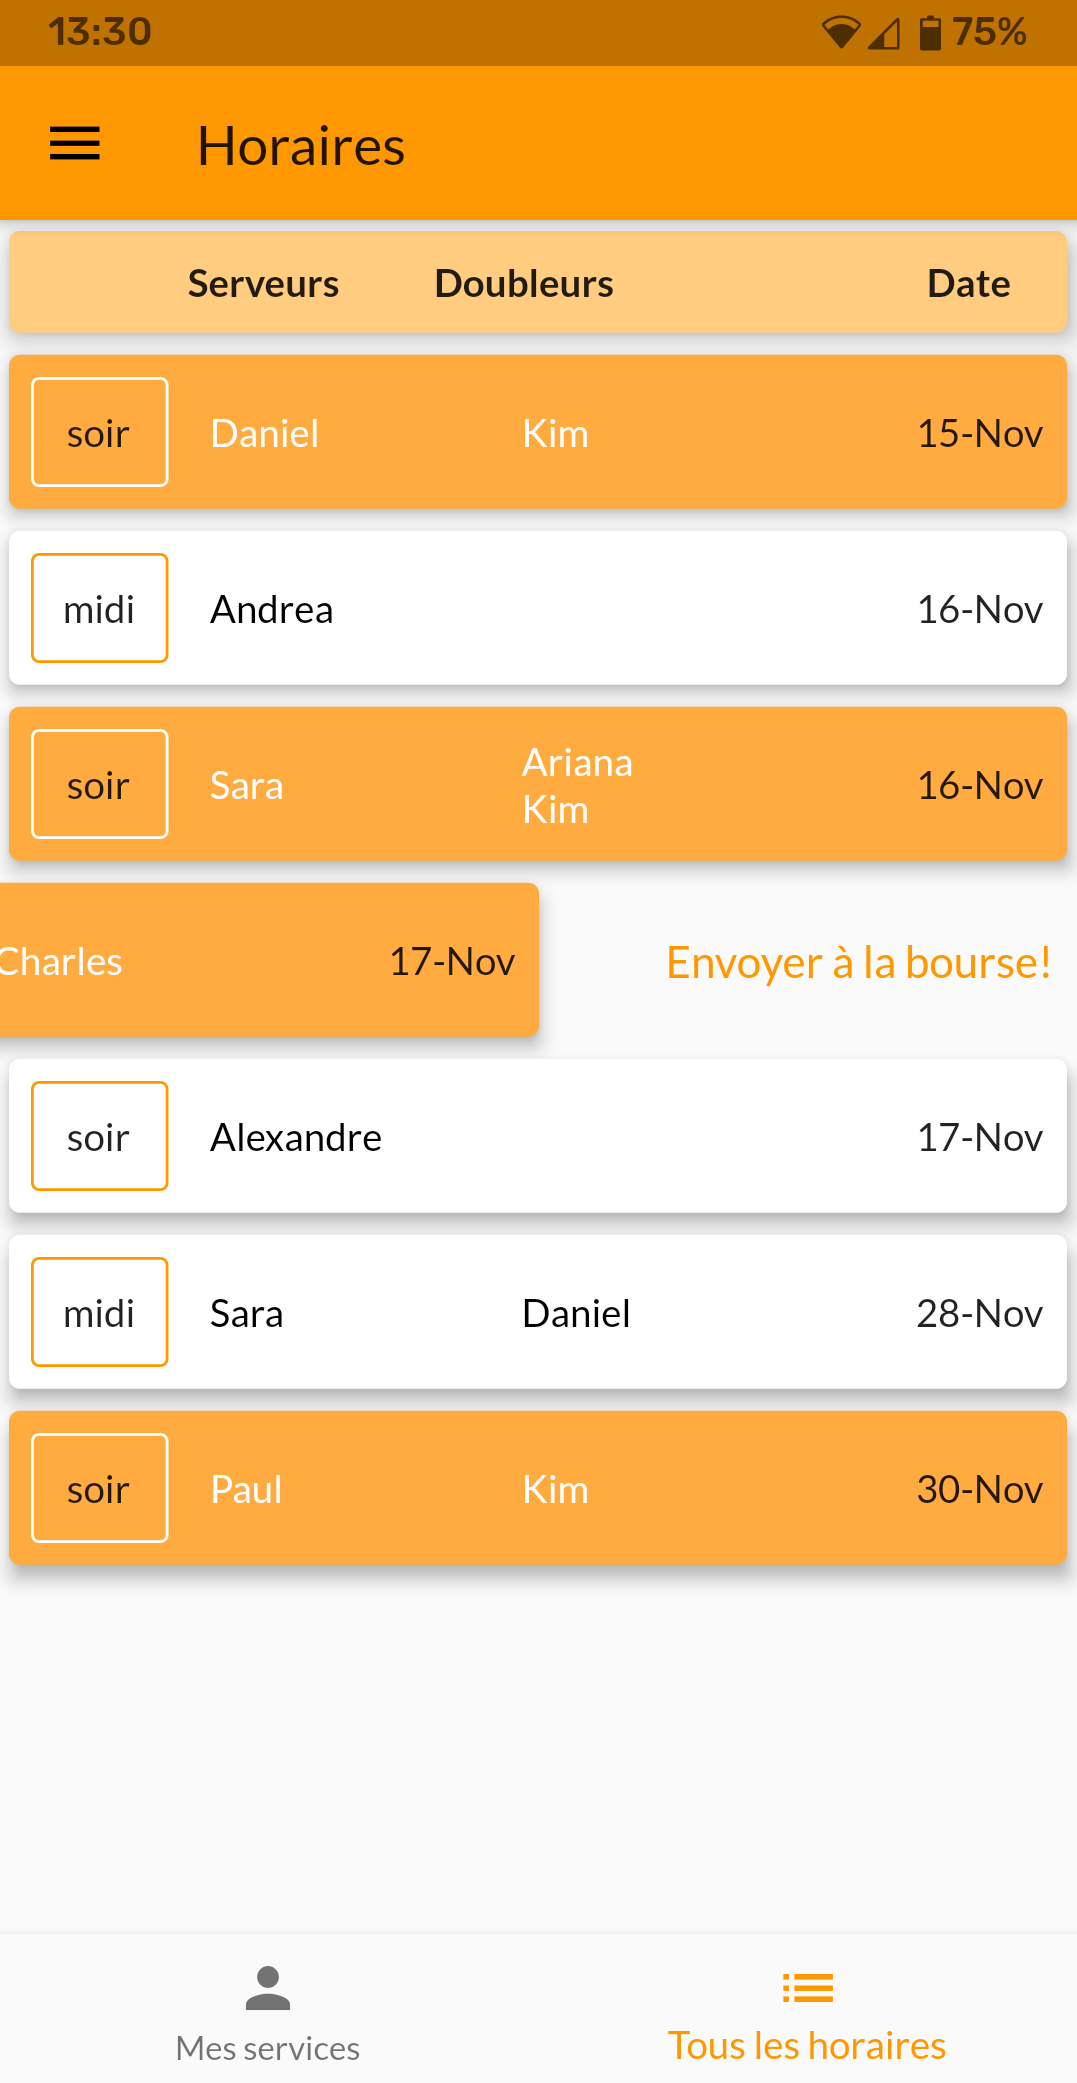
\includegraphics[width=0.9\linewidth]{screenshots/scenario_02/mise_en_bourse.png}
            \caption{mise en bourse}
            \label{fig:mise_en_bourse}
        \end{subfigure}
        \begin{subfigure}{.3\textwidth}
            \centering
            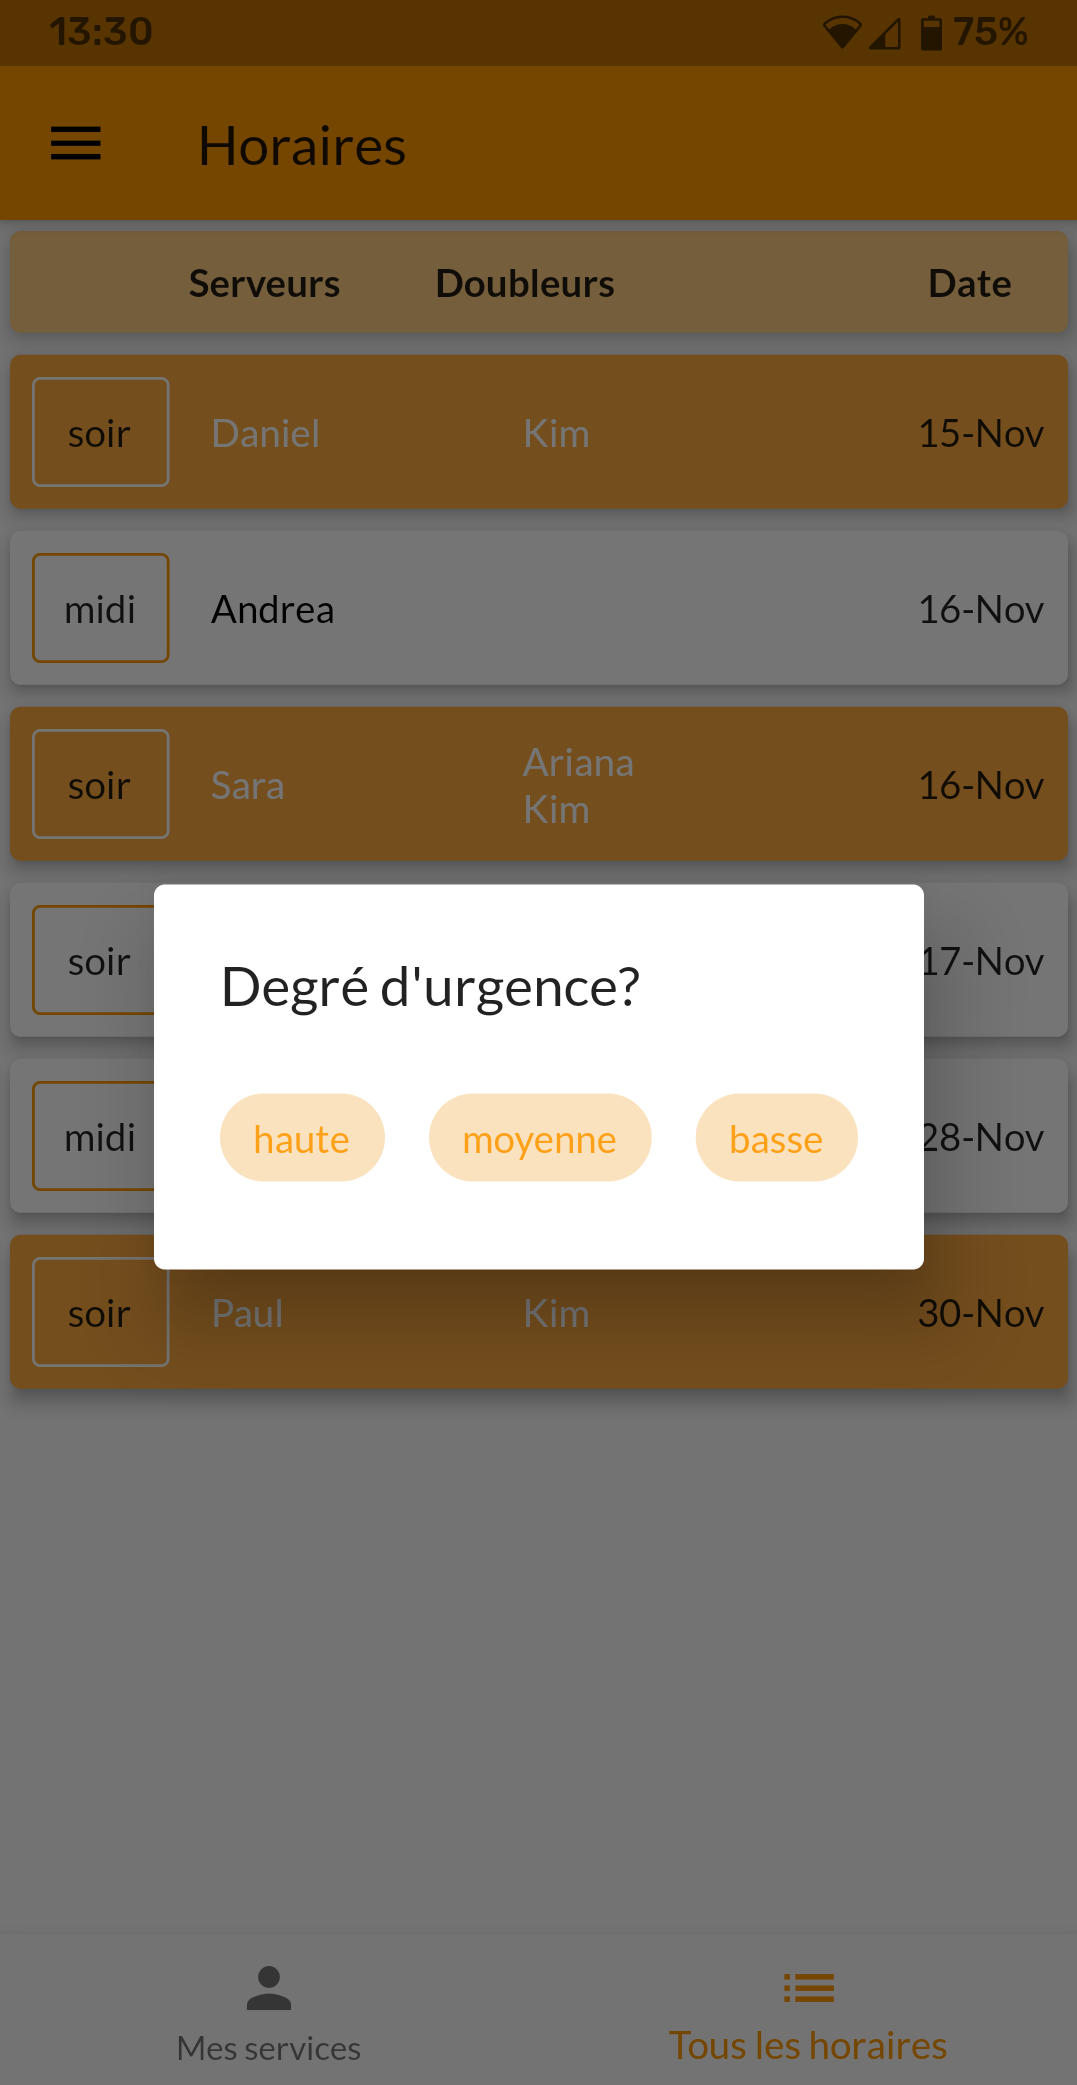
\includegraphics[width=0.9\linewidth]{screenshots/scenario_02/urgence.png}
            \caption{urgence}
            \label{fig:urgence}
        \end{subfigure}
        \begin{subfigure}{.3\textwidth}
            \centering
            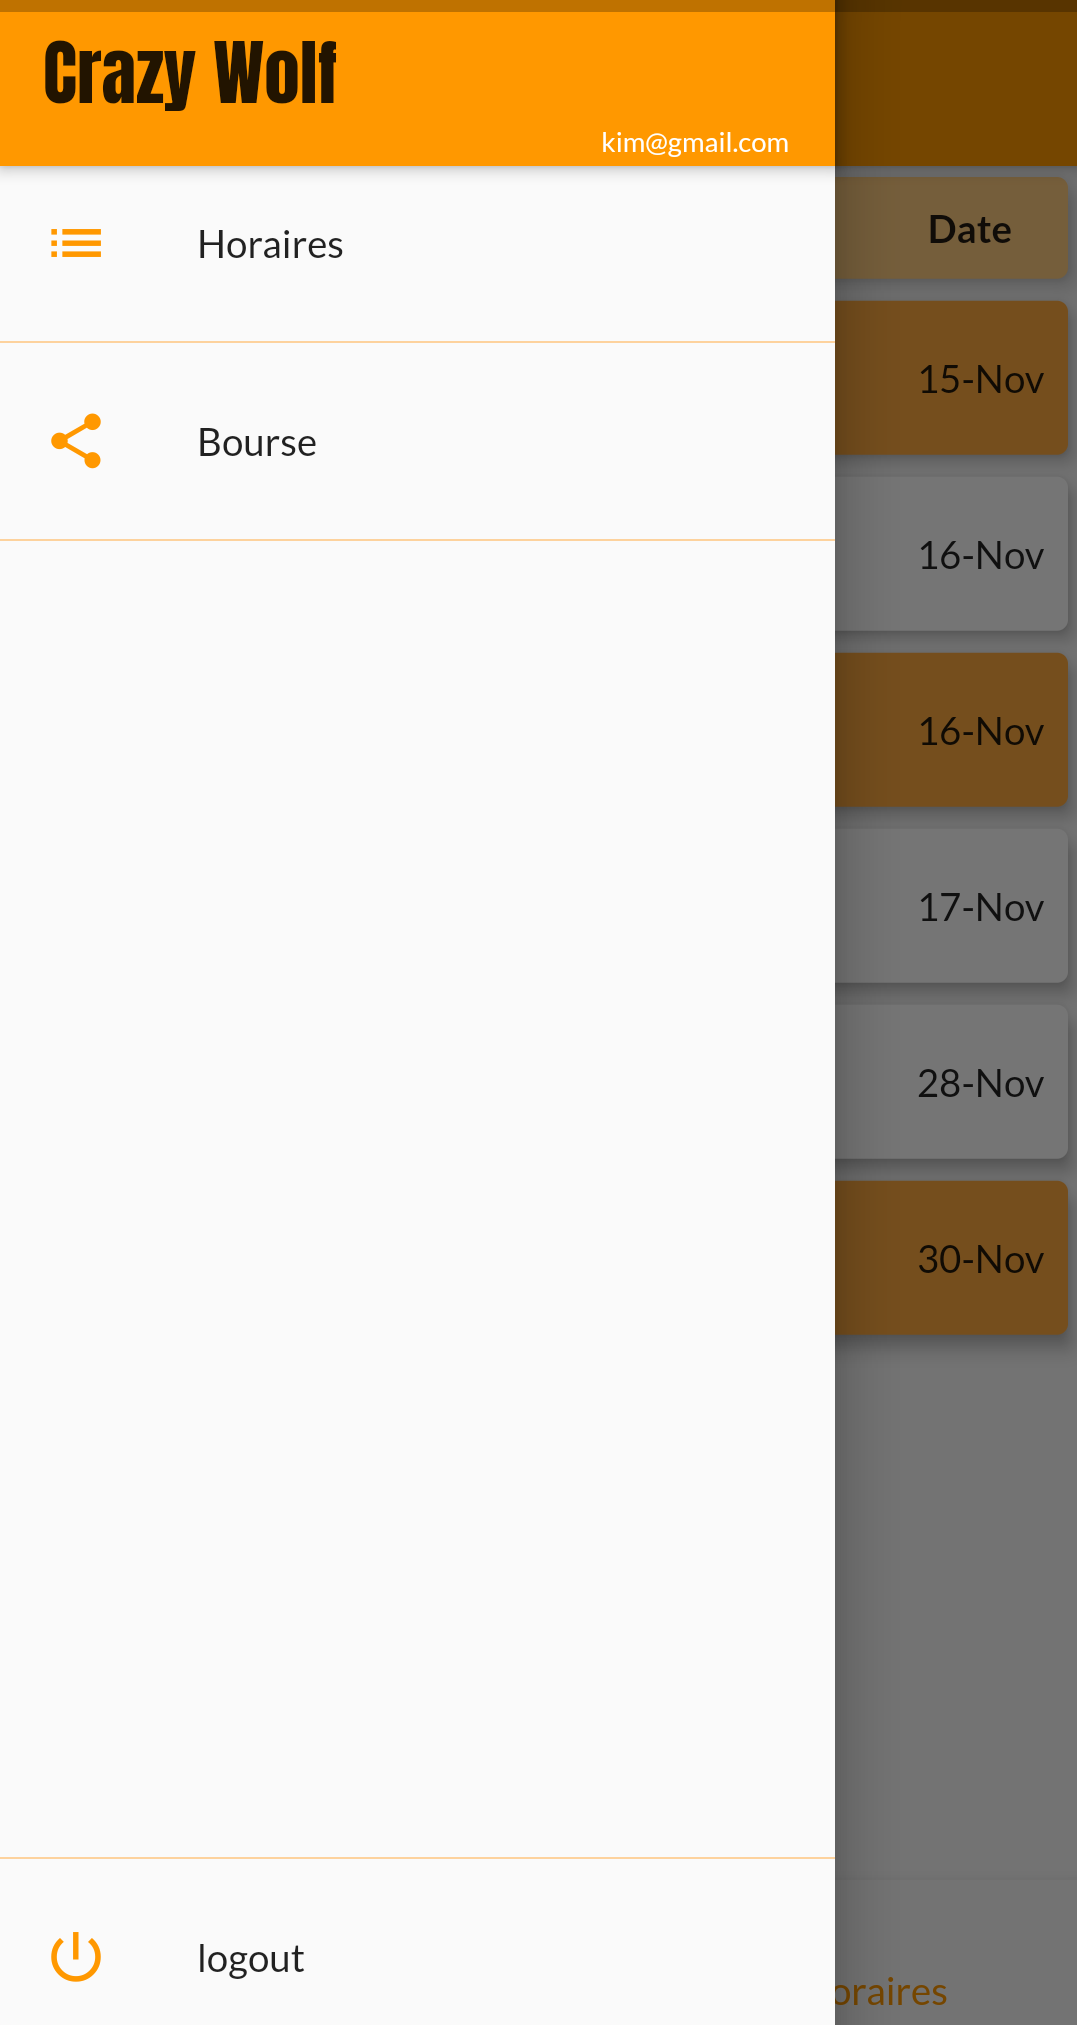
\includegraphics[width=0.9\linewidth]{screenshots/scenario_02/menu_serveur_normal.png}
            \caption{menu sans privilèges}
            \label{fig:menu_sans_droits}
        \end{subfigure}
        \caption{scénario II - a}
        \label{fig:scen02a}
    \end{figure}

Une fois le glissement effectué un popup est s'affiche \ref{fig:urgence} demandant
à quel point le remplacement est urgent. Une fois que l'utilisateur à répondu, le service est mis
en bourse. Un snakbar \footnote{Petite notification informative qui émerge dans la partie inférieur d'un écran} s'affiche pour le notifier que l'action à réussi.

Si l'action est réussie, tous les utilisateurs de l'application sont notifiés \ref{fig:notif} comme quoi un 
nouveau service est disponible. La notification informe sur la disponibilité d'un service ainsi que 
l'urgence requise à y répondre.

Suit à ça, l'utilisatrice peut naviguer à l'aide du menu latéral \ref{fig:menu_sans_droits} où s'affichent les options
de navigation suivante:
\smallskip
\begin{itemize}
    \item Horaires: Pour aller à l'écran \textit{Horaires} \ref{fig:horaires}
    \item Logout: Pour se déconnecter, qui renvoie à l'écran \ref{fig:login} d'authentification
    \item Bourse: Pour aller à l'écran \textit{Bourse aux jobs} \ref{fig:bourse}
\end{itemize}

\newpage
Dans l'onglet \textit{Bourse aux jobs} \ref{fig:bourse} son service est disponible à toute personne souhaitant y postuler. 
Cet onglet est partagé parmi tous les utilisateurs de l'application.

\begin{figure}[!h]
    \centering
    \begin{subfigure}[]{.3\textwidth}
        \centering
        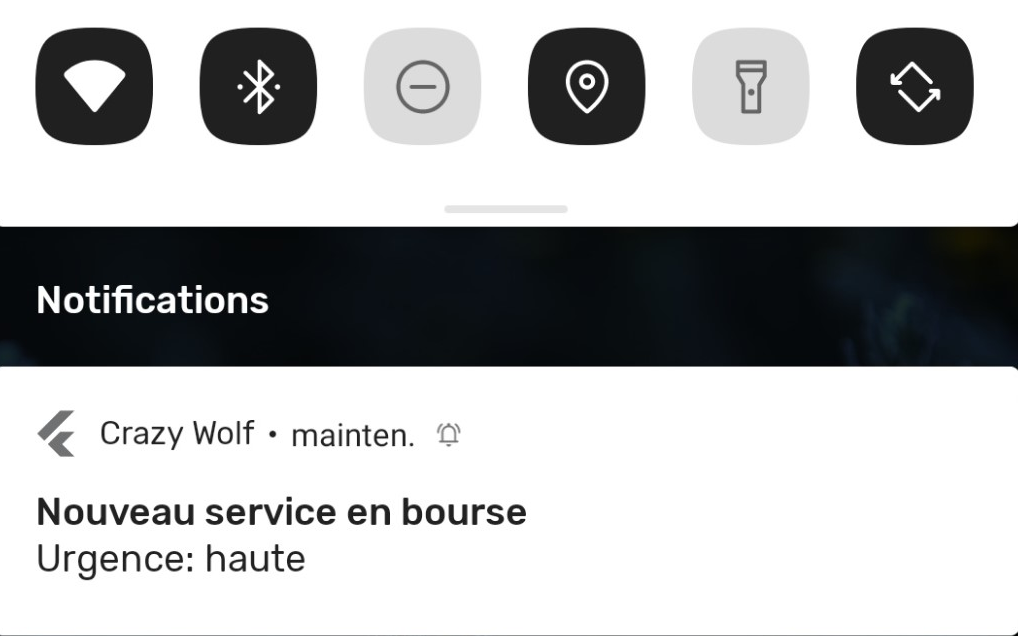
\includegraphics[width=0.9\linewidth]{screenshots/scenario_02/notification.png}
        \caption{notification}
        \label{fig:notif}
    \end{subfigure}
    \begin{subfigure}{.3\textwidth}
        \centering
        
\includegraphics[width=0.9\linewidth]{screenshots/scenario_02/bourse_jobs.png}
        \caption{bourse}
        \label{fig:bourse}
    \end{subfigure}
    \caption{scénario II - b}
    \label{fig:scen02b}
\end{figure}

La couleur représente le degré d'urgence. Ainsi la convention suivante est appliqué:
\smallskip
\begin{itemize}
    \item rouge: implique une urgence élevée.
    \item jaune: implique une urgence moyenne.
    \item vert: implique une urgence basse.
\end{itemize}
\smallskip
L'onglet \textit{Bourse aux jobs} affiche tous les service actuellement en bourse sous
forme de liste scrollable. L'utilisateur ayant mis son service en bourse
doit patienter à ce que quelqu'un y postule.

Les utilisateur sans privilèges sont autorisé à mettre un service en bourse uniquement s'ils y travaillent.

\section[Postuler pour un service - Scénario III]{Scénario III}
    \subsection*{Postuler pour un service}
    Dans la continuation du scénario précédent, après avoir été notifiés,
    deux serveurs vont postuler au nouveau service mis
    en bourse. Leurs parcours étant identiques, nous allons en montrer qu'un.
    Supposons qu'ils se soient authentifié comme vu en \ref{fig:login} et qu'ils se trouvent
    dans l'onglet \textit{Bourse au jobs} \ref{fig:bourse}.
    \vfill
    \begin{figure}[h]
        \centering
        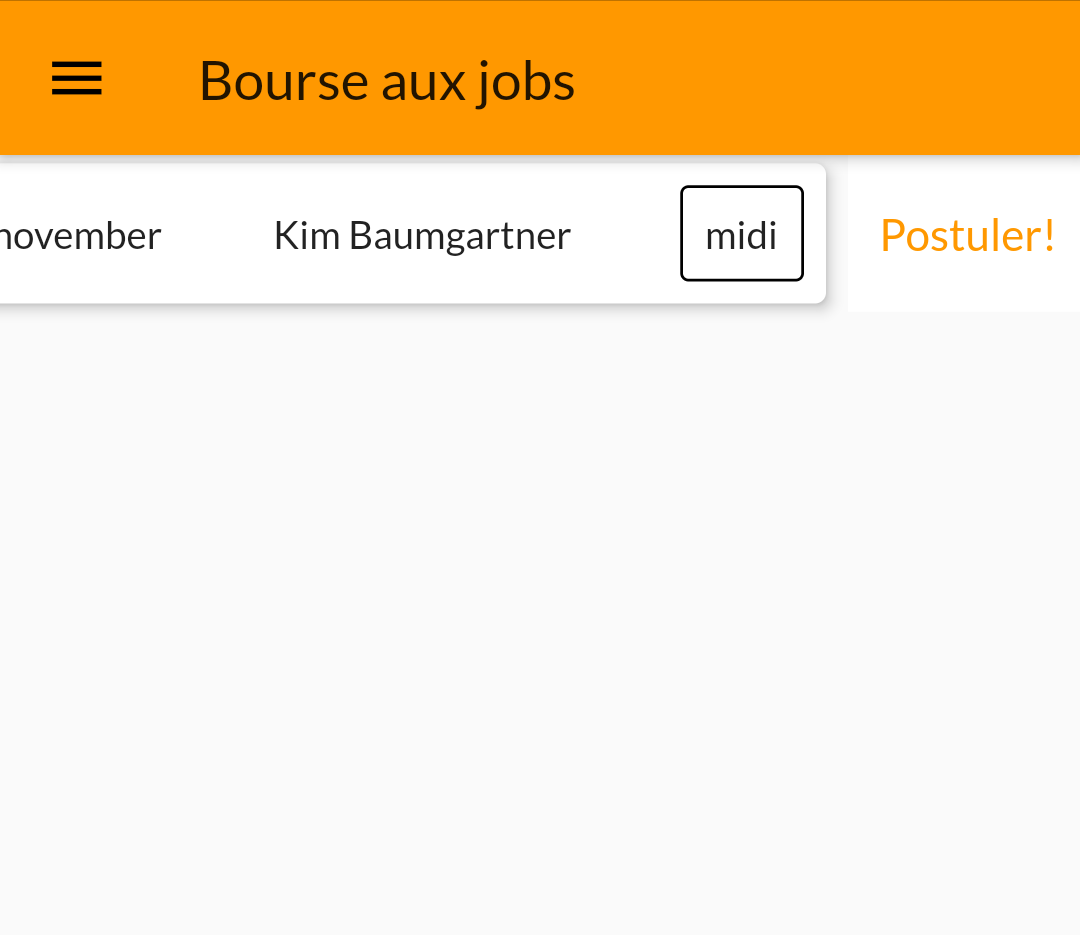
\includegraphics[width=.3\linewidth]{screenshots/scenario_03/postuler.png}
        \caption{postuler}
        \label{fig:postuler}
    \end{figure}
    \vfill
    Alors, ils peuvent glisser le service auquel ils souhaitent postuler sur
    la gauche \ref{fig:postuler}. À nouveau, si l'opération réussi, un snackbar apparaît pour l'indiquer.
    \newpage
    L'utilisateur ayant mis le service en bourse doit procéder à l'acceptation
    d'un seul postulant. Dans \textit{Bourse aux jobs} \ref{fig:bourse} les éléments de 
    la liste sont clicable. Lorsqu'un utilisateur clic deux options sont possibles:
    \smallskip
    \begin{figure}[!h]
        \centering
        \begin{subfigure}{.3\textwidth}
            \centering
            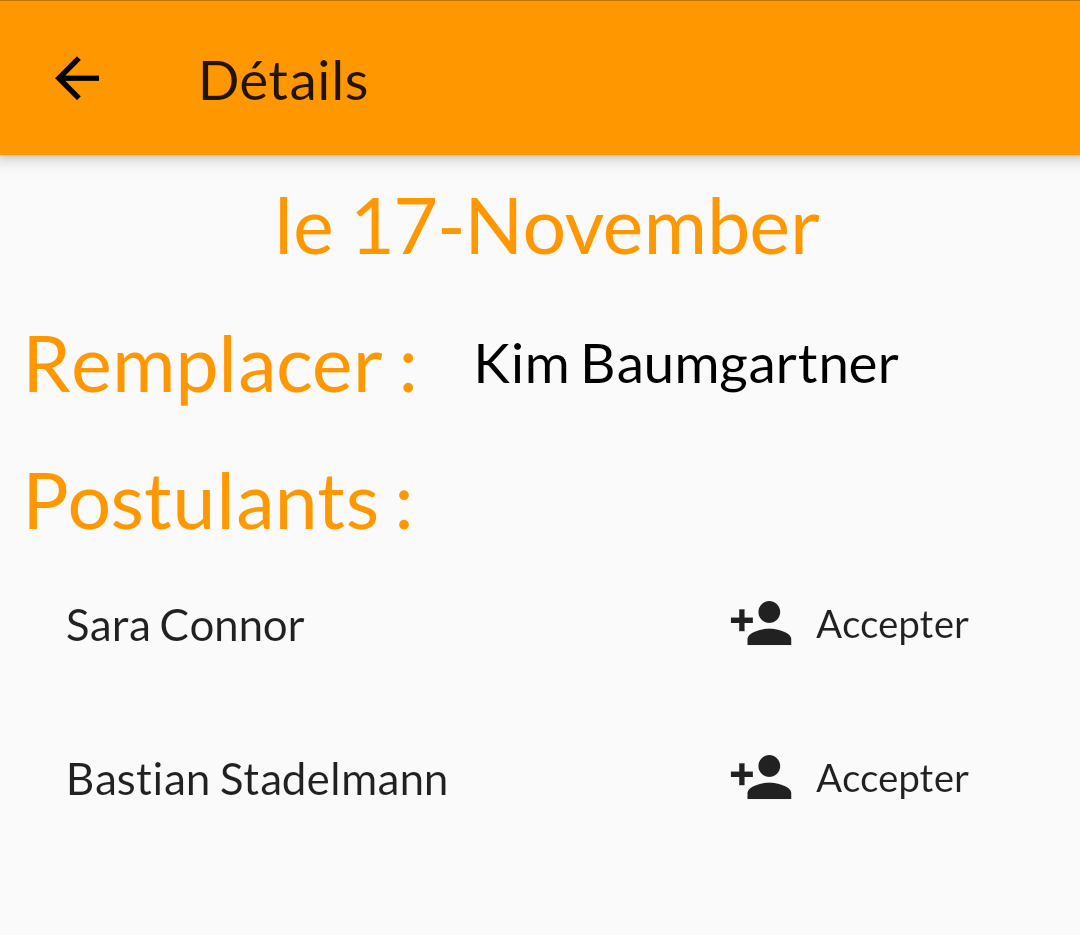
\includegraphics[width=0.9\linewidth]{screenshots/scenario_03/detail_auth.png}
            \caption{kim}
            \label{fig:detail_auth}
        \end{subfigure}
        \begin{subfigure}{.3\textwidth}
            \centering
            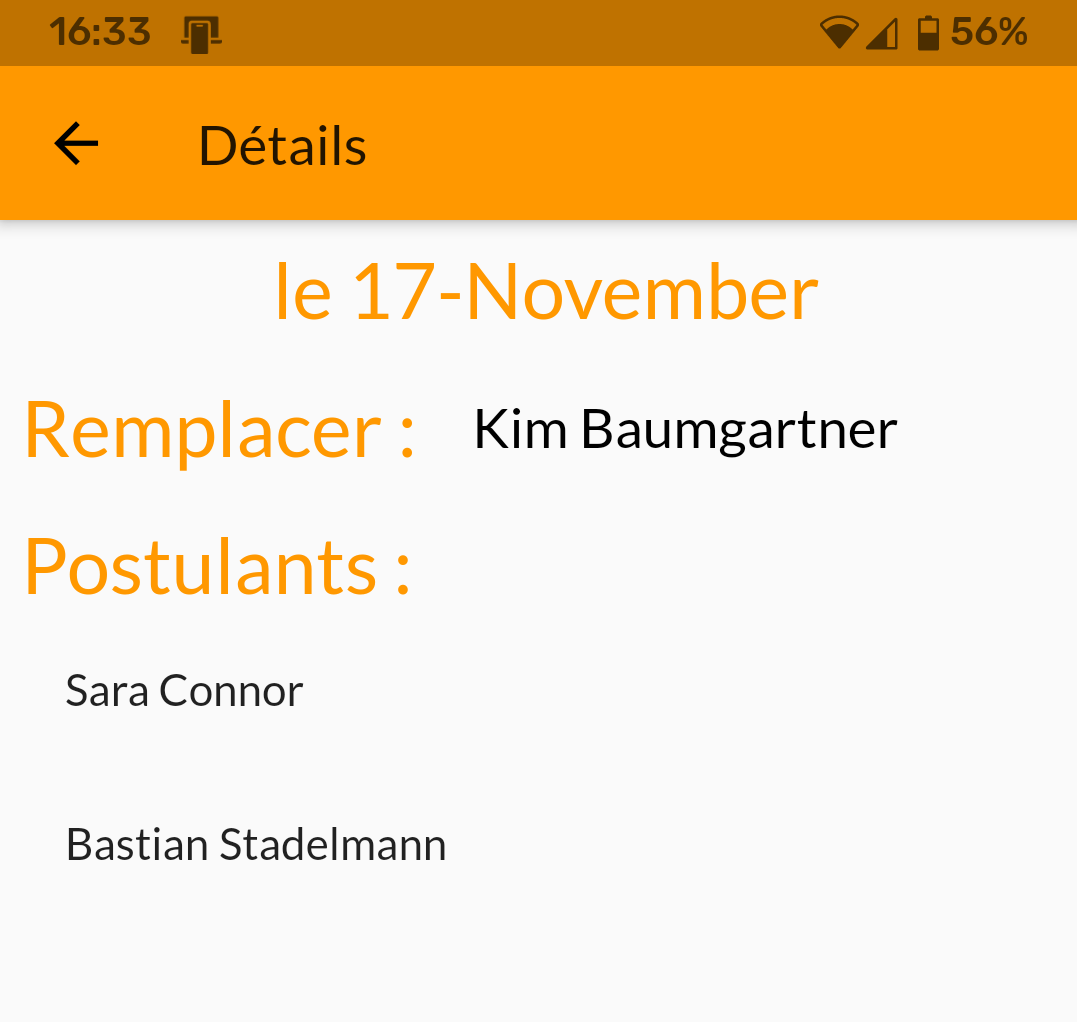
\includegraphics[width=0.9\linewidth]{screenshots/scenario_03/detail_non_auth.png}
            \caption{autre}
            \label{fig:detail_non_auth}
        \end{subfigure}
        \begin{subfigure}{.3\textwidth}
            \centering
            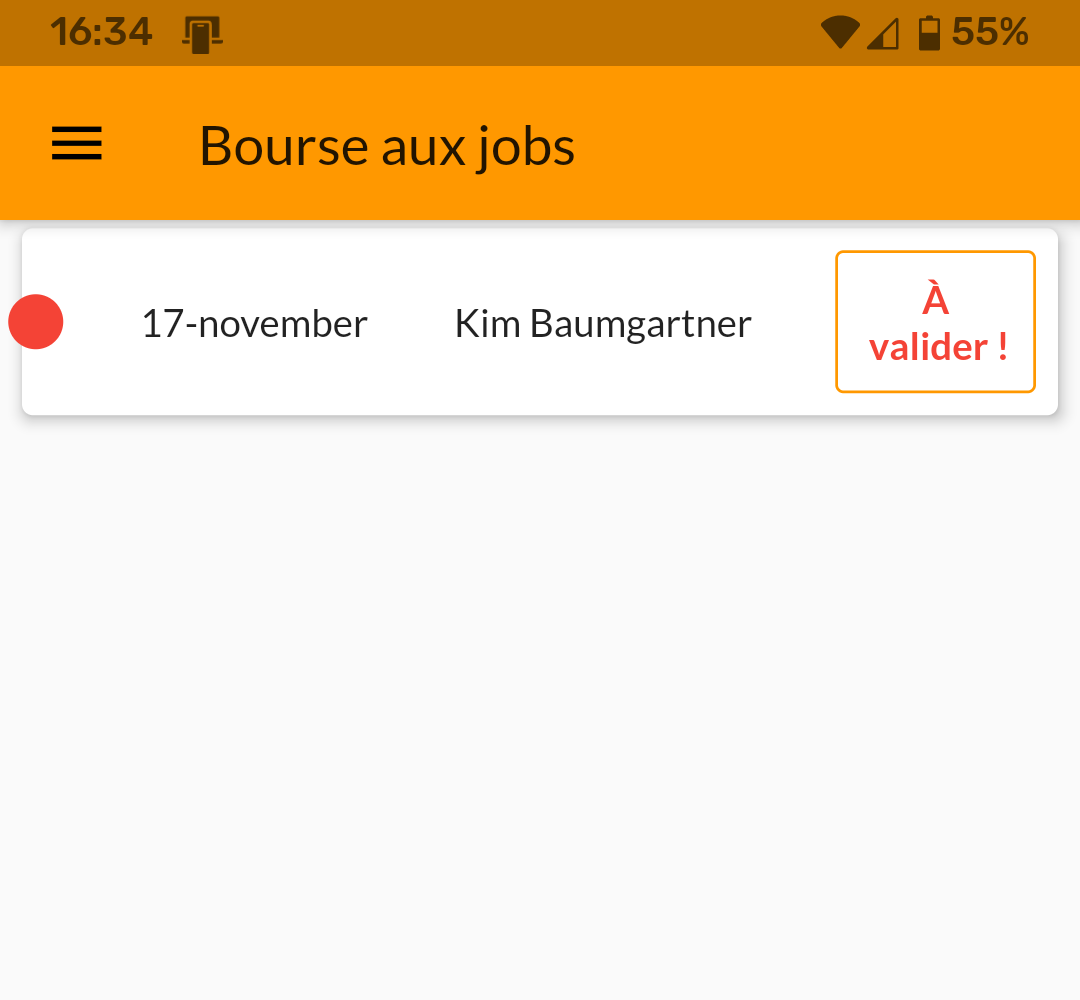
\includegraphics[width=0.9\linewidth]{screenshots/scenario_03/a_valider.png}
            \caption{à valider}
            \label{fig:a_valider}
        \end{subfigure}
        \caption{scénario III}
        \label{fig:scen03}
    \end{figure}

    S'il s'agit de l'utilisateur ayant mis le service en bourse à l'occurrence Kim, l'écran \textit{Détails} tel que \ref{fig:detail_auth} s'affiche.
    
    S'il s'agit de n'importe quel autre utilisateur alors l'écran \textit{Détails} s'affiche comme dans \ref{fig:detail_non_auth}

    Ainsi, seul l'utilisateur ayant mis le service en bourse est en mesure d'accepter un ou une remplaçante. 
    
    Pour se faire, Kim doit appuyer sur le bouton \textit{accepter} de la personne de son choix.
    Elle accepte Sara. Tous les utilisateurs ayant des privilèges sont notifiés qu'un service nécéssite validation.
    En attendant, l'élément de la bourse dans \textit{Bourse aux jobs} \ref{fig:a_valider} s'affiche comme nécéssitant validation.

\section[Valider un échange - Scénario IV]{Scénario IV}
    \subsection*{Valider un échange}
    Toujours dans la continuation de notre exemple, nous allons voir ici 
    la validation d'un échange. En effet, même si un utilisateur
    a accepté un remplaçant pour son service. Il faut encore que cette
    transaction soit validée par un utilisateur avec des privilèges.

    Il existe trois types d'utilisateurs:
    \begin{center}
        \begin{tikzpicture}
            \node[] at (0.5,2) {normal};
            \draw[color=RoyalRed] (2,2) circle (3.5cm);
            \node[] at (2.5,1.5) {manager};
            \draw[color=RoyalRed] (1,2) circle (2.5cm);
            \node[] at (4.5,1.0) {admin};
            \draw[color=RoyalRed] (0,2) circle (1.5cm);
        \end{tikzpicture}
    \end{center}

    Les utilisateurs autres que \textit{normal} ont des privilèges.

    \begin{itemize}
        \item [Normal:] Peut demander un échange et accepter des postulants.
        \item [Manager:] Peut valider un échange, créer des services et demander des doubleurs en renfort.
        \item [Admin:] Peut ajouter de nouveaux serveurs. 
    \end{itemize}
    
    Lorsque l'on clic sur l'élément à valider \ref{fig:a_valider} deux options
    sont possibles suivant si l'utilisateur authentifié \ref{fig:valider_manager} et \textit{manager / admin} ou bien 
    s'il est \textit{normal} \ref{fig:attente_validation}.

    \begin{figure}[!h]
        \centering
        \begin{subfigure}{.3\textwidth}
            \centering
            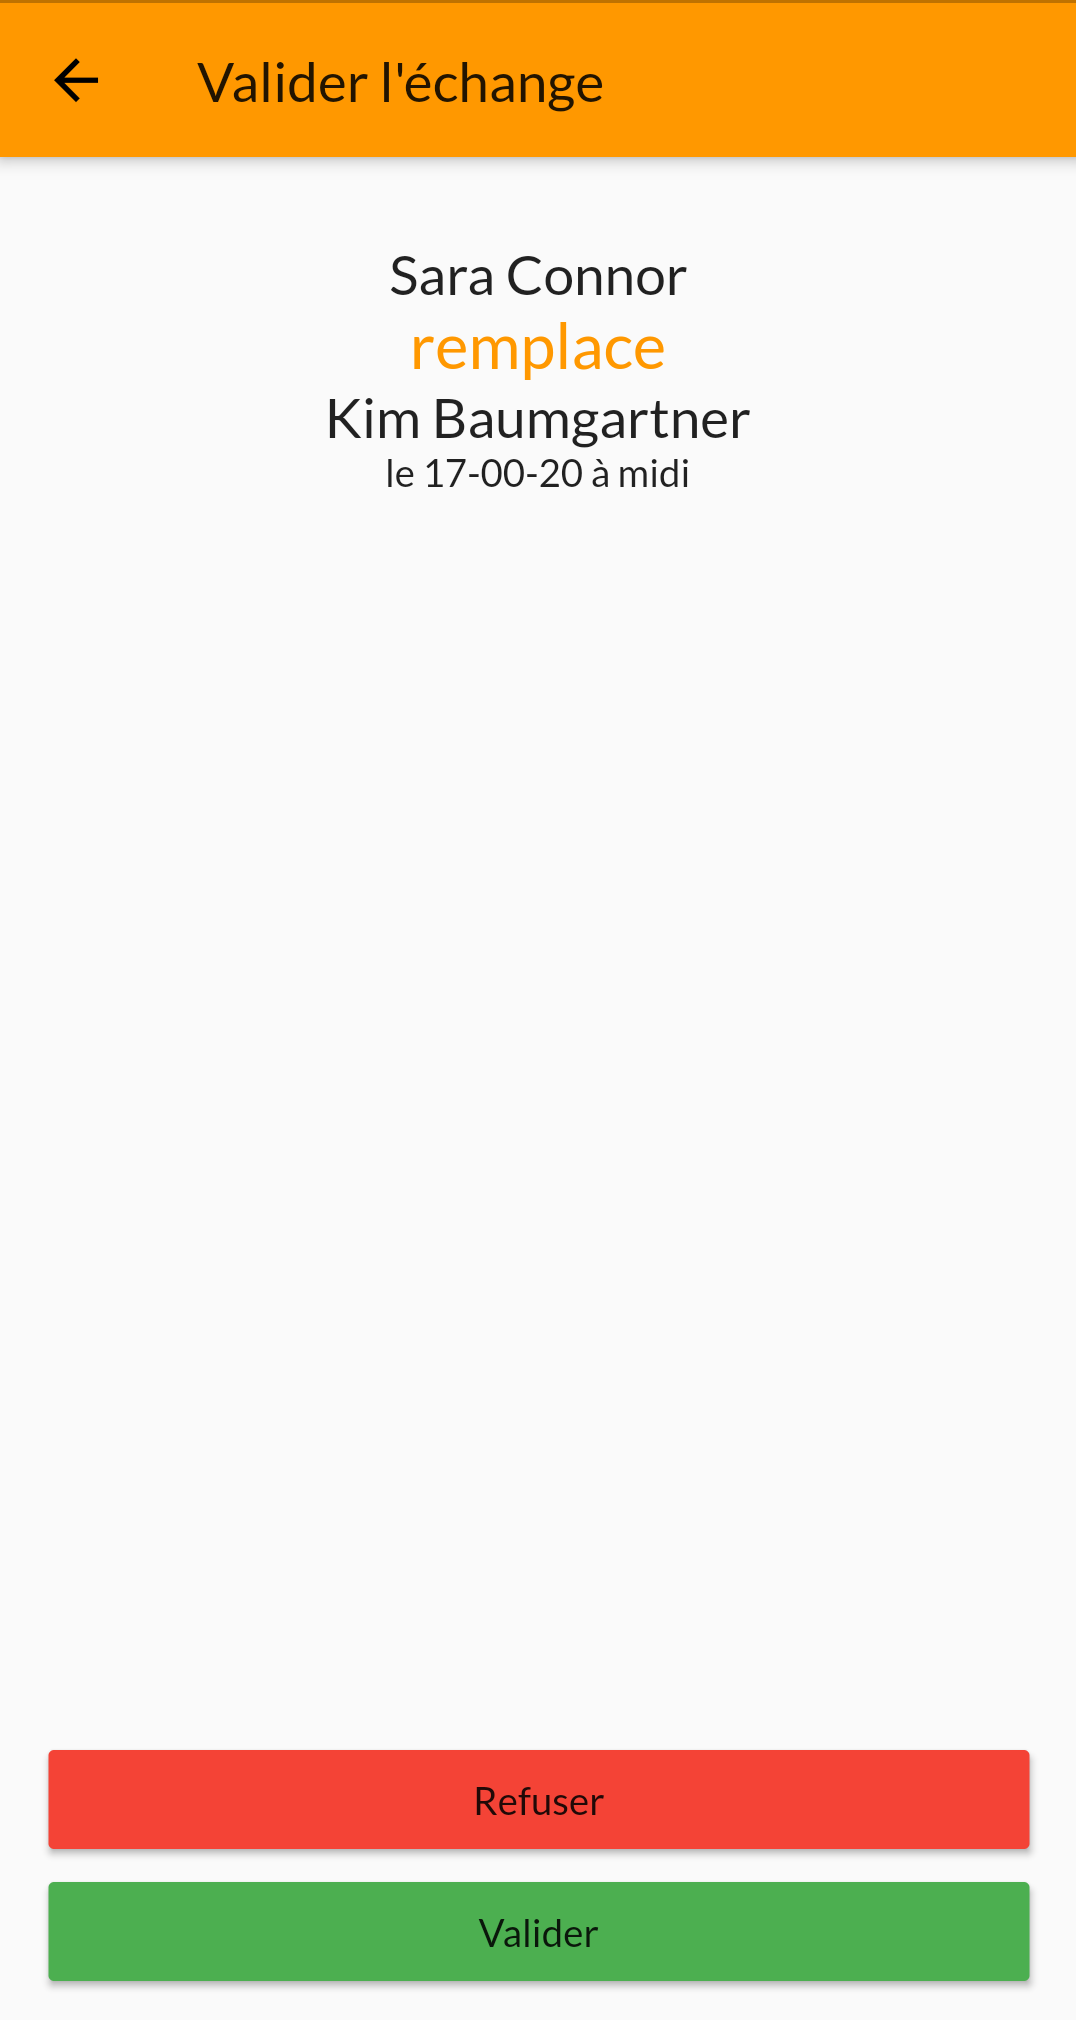
\includegraphics[width=0.9\linewidth]{screenshots/scenario_04/valider_manager.png}
            \caption{manager / admin}
            \label{fig:valider_manager}
        \end{subfigure}
        \begin{subfigure}{.3\textwidth}
            \centering
            
\includegraphics[width=0.9\linewidth]{screenshots/scenario_04/en_attente_validation.png}
            \caption{normal}
            \label{fig:attente_validation}
        \end{subfigure}
        \begin{subfigure}{.3\textwidth}
            \centering
            \includegraphics[width=0.9\linewidth]{screenshots/scenario_04/validé.png}
            \caption{Daniel: après validation}
            \label{fig:validé}
        \end{subfigure}
        \caption{scénario IV}
        \label{fig:scen04}
    \end{figure}

S'il s'agit d'un utilisateur avec privilèges, alors il a l'option de valider l'échange \ref{fig:valider_manager}. 

Supposons que Daniel, qui est administrateur valide l'échange. Alors, l'écran \textit{Horaires} est modifié \ref{fig:validé}
pour tout le monde et affiche que c'est bien Sara qui travail le 17 novembre et non plus Kim. 

De plus, l'élément dans \textit{Bourse aux jobs} \ref{fig:bourse} est supprimé.
\newpage
\section[Ajouter un service - Scénario V]{Scénario V}
    \subsection*{Ajouter un service}
    Afin de créer les horaires pour le personnel, un manager ou administrateur doit créer des services. Supposons
    que c'est Ari, une manager qui le fait. Après s'être authentifiée, elle peut à l'aide du menu latéral \ref{fig:menu_manager} naviguer
    à \textit{Ajouter service} \ref{fig:ajout_service}

    \begin{figure}[!h]
        \centering
        \begin{subfigure}{.3\textwidth}
            \centering
            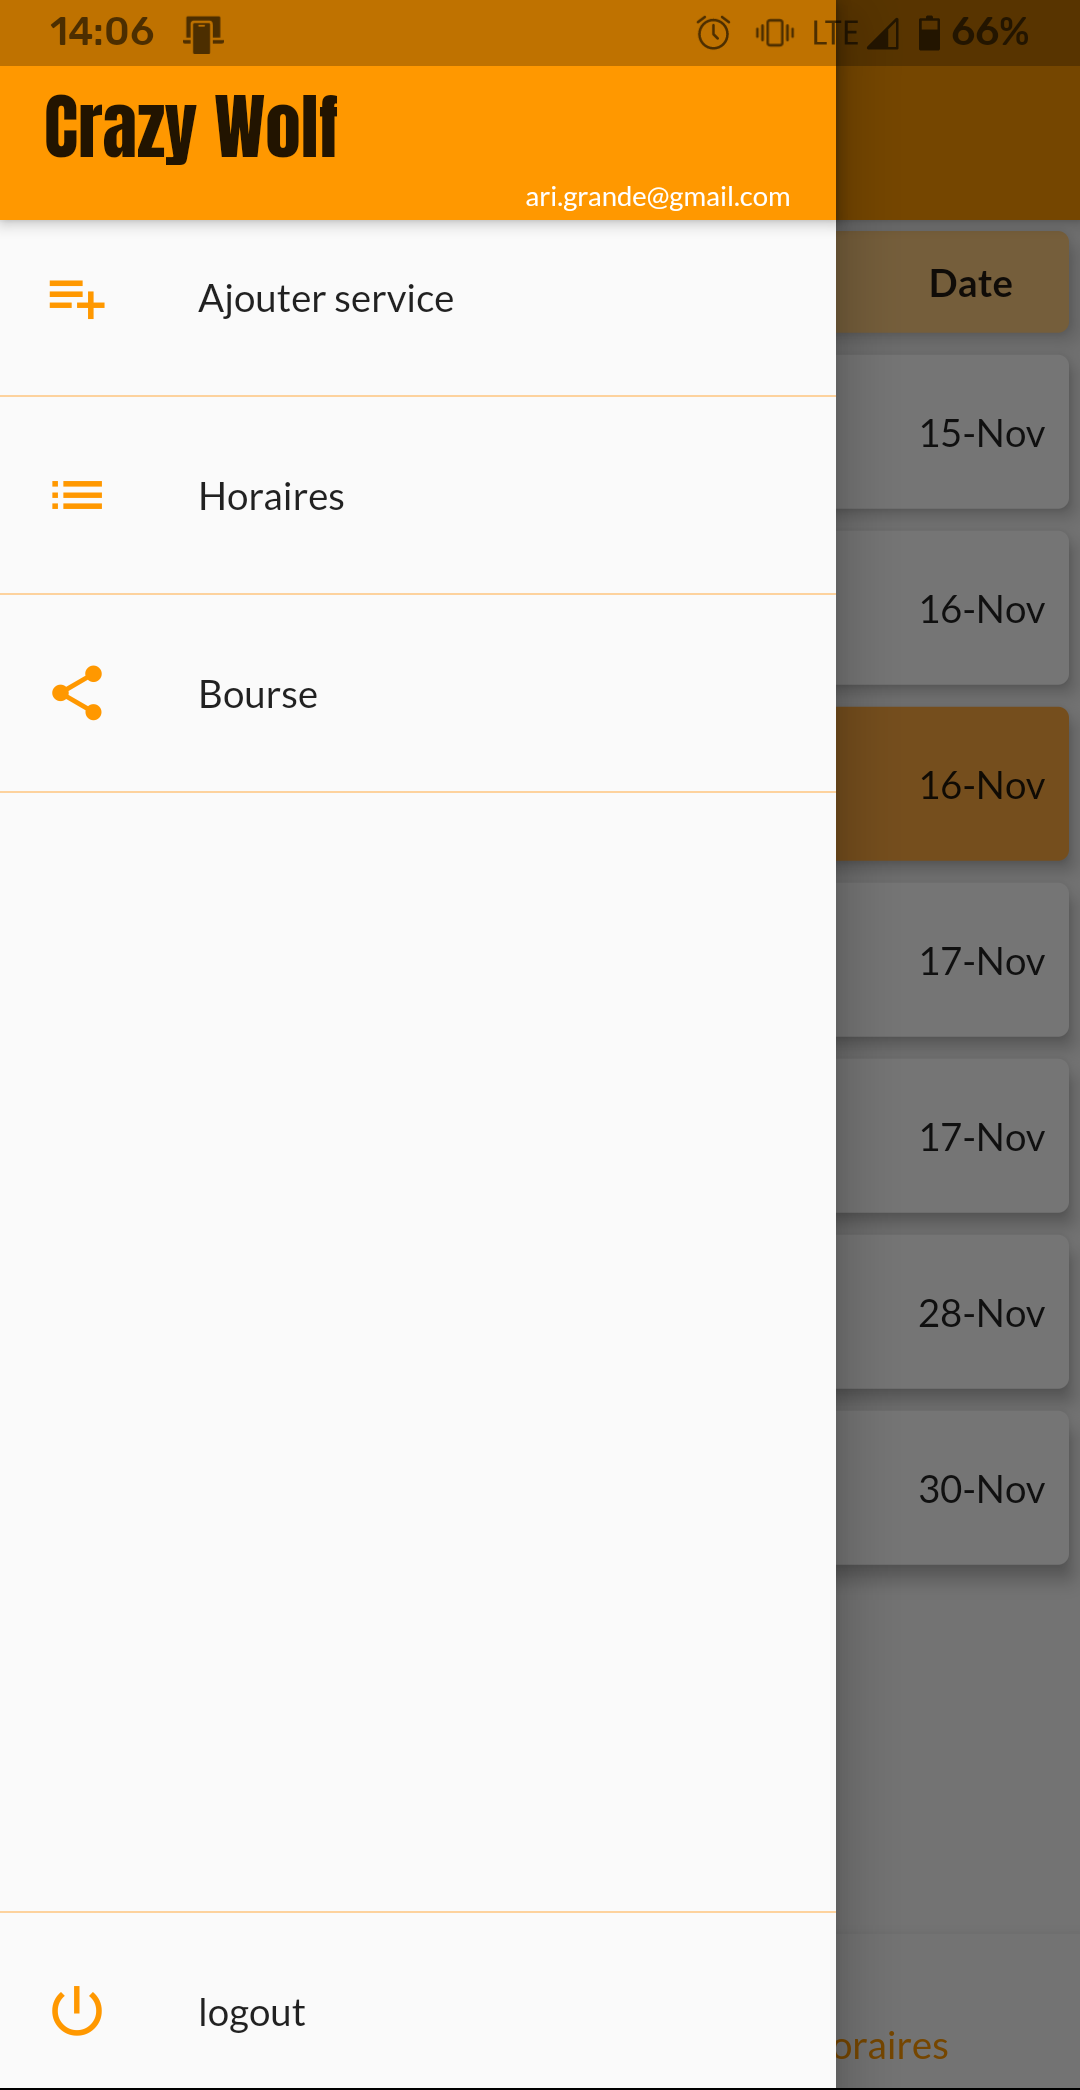
\includegraphics[width=0.9\linewidth]{screenshots/scenario_05/menu_manager.png}
            \caption{menu manager}
            \label{fig:menu_manager}
        \end{subfigure}
        \begin{subfigure}{.3\textwidth}
            \centering
            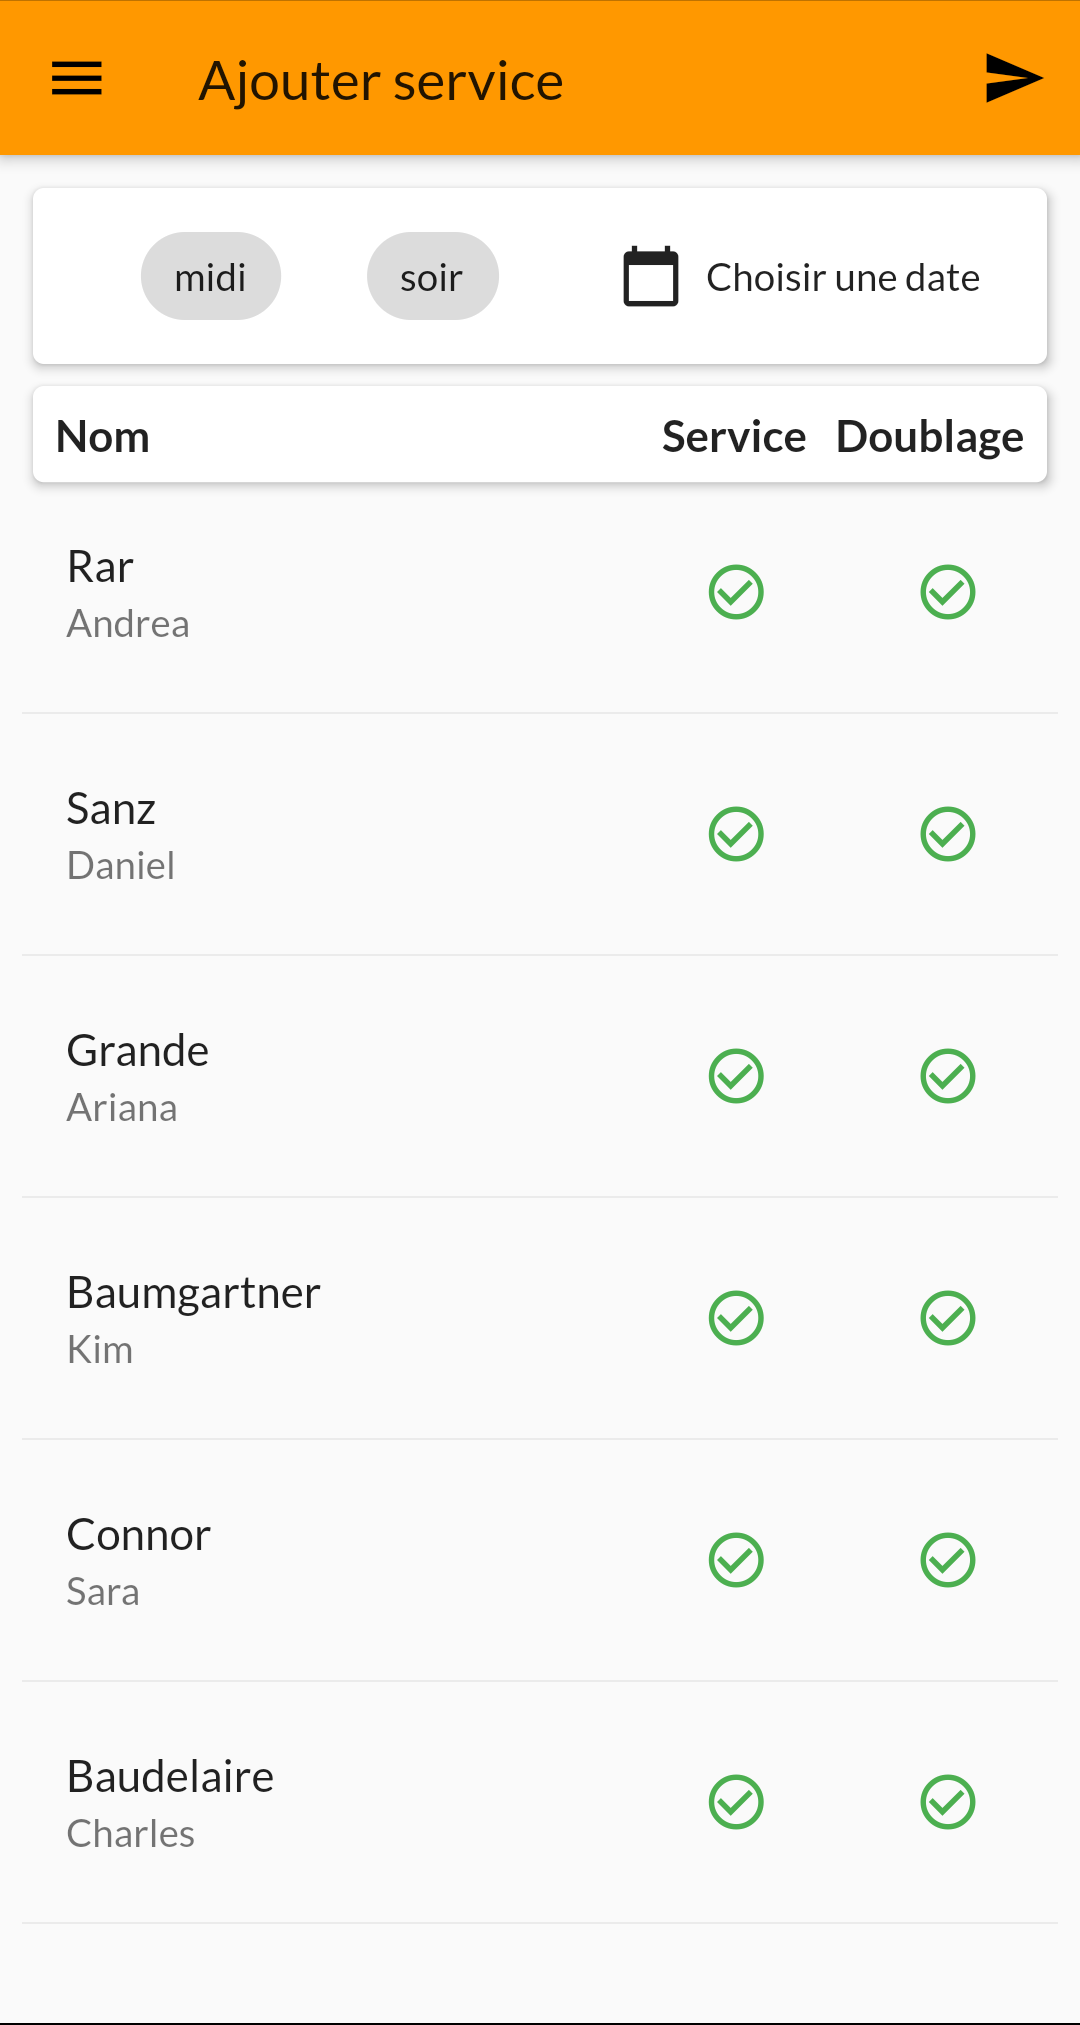
\includegraphics[width=0.9\linewidth]{screenshots/scenario_05/ajout_service_a.png}
            \caption{ajouter service}
            \label{fig:ajout_service}
        \end{subfigure}
        \begin{subfigure}{.3\textwidth}
            \centering
            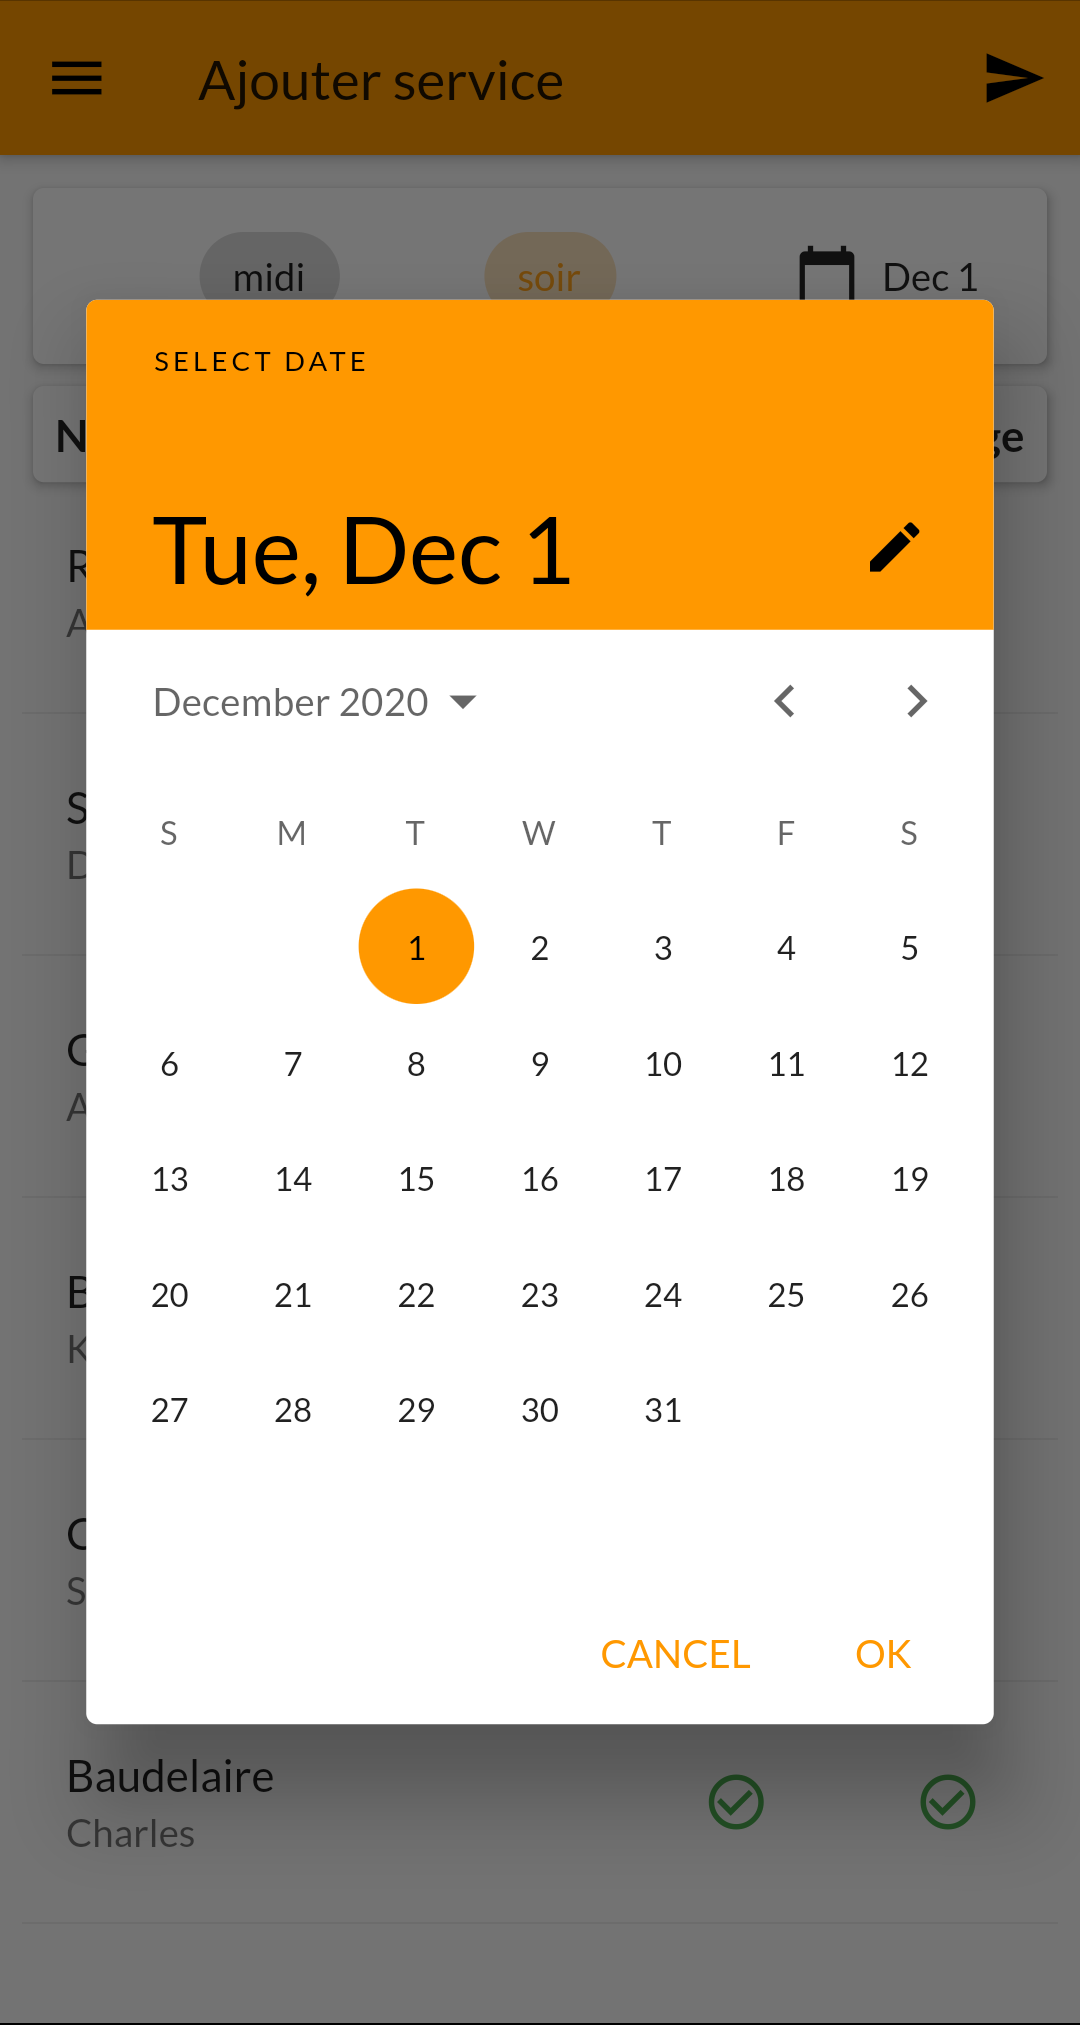
\includegraphics[width=0.9\linewidth]{screenshots/scenario_05/ajout_service_b.png}
            \caption{choix date}
            \label{fig:choix_date}
        \end{subfigure}
        \caption{scénario V - a}
        \label{fig:scen05a}
    \end{figure}

    Pour créer le service, il faut choisir:
    \smallskip
    \begin{itemize}
        \item une date en appuyant sur \textit{Choisir une date} un popup avec le calendrier s'affiche \ref{fig:choix_date}.
        \item un type en appuyant sur \textit{midi} ou \textit{soir} \ref{fig:ajout_service_c}. 
        \item une ou plusieurs personnes au \textit{Service} \ref{fig:ajout_service_c}.
        \item zéro, une ou plusieurs personnes au \textit{Doublage} \ref{fig:ajout_service_c}.
    \end{itemize}
    
    \newpage
    Dans notre exemple Ari choisit le 1er décembre au soir. Andrea au service et Daniel au doublage.

    Un service ne peut pas avoir la même personne au doublage et au service. Un service peut ne pas avoir
    de doubleurs. 

    De plus, l'opération ajouter le service aux horaires qui se fait au moyen du bouton envoyer
    dans le coin supérieur droit de la figure \ref{fig:ajout_service_c} retournera une erreur s'il existe un 
    service du même type à la même date.

    \begin{center}
    \begin{figure}[h]
        \centering
        \begin{subfigure}{.45\textwidth}
            \centering
            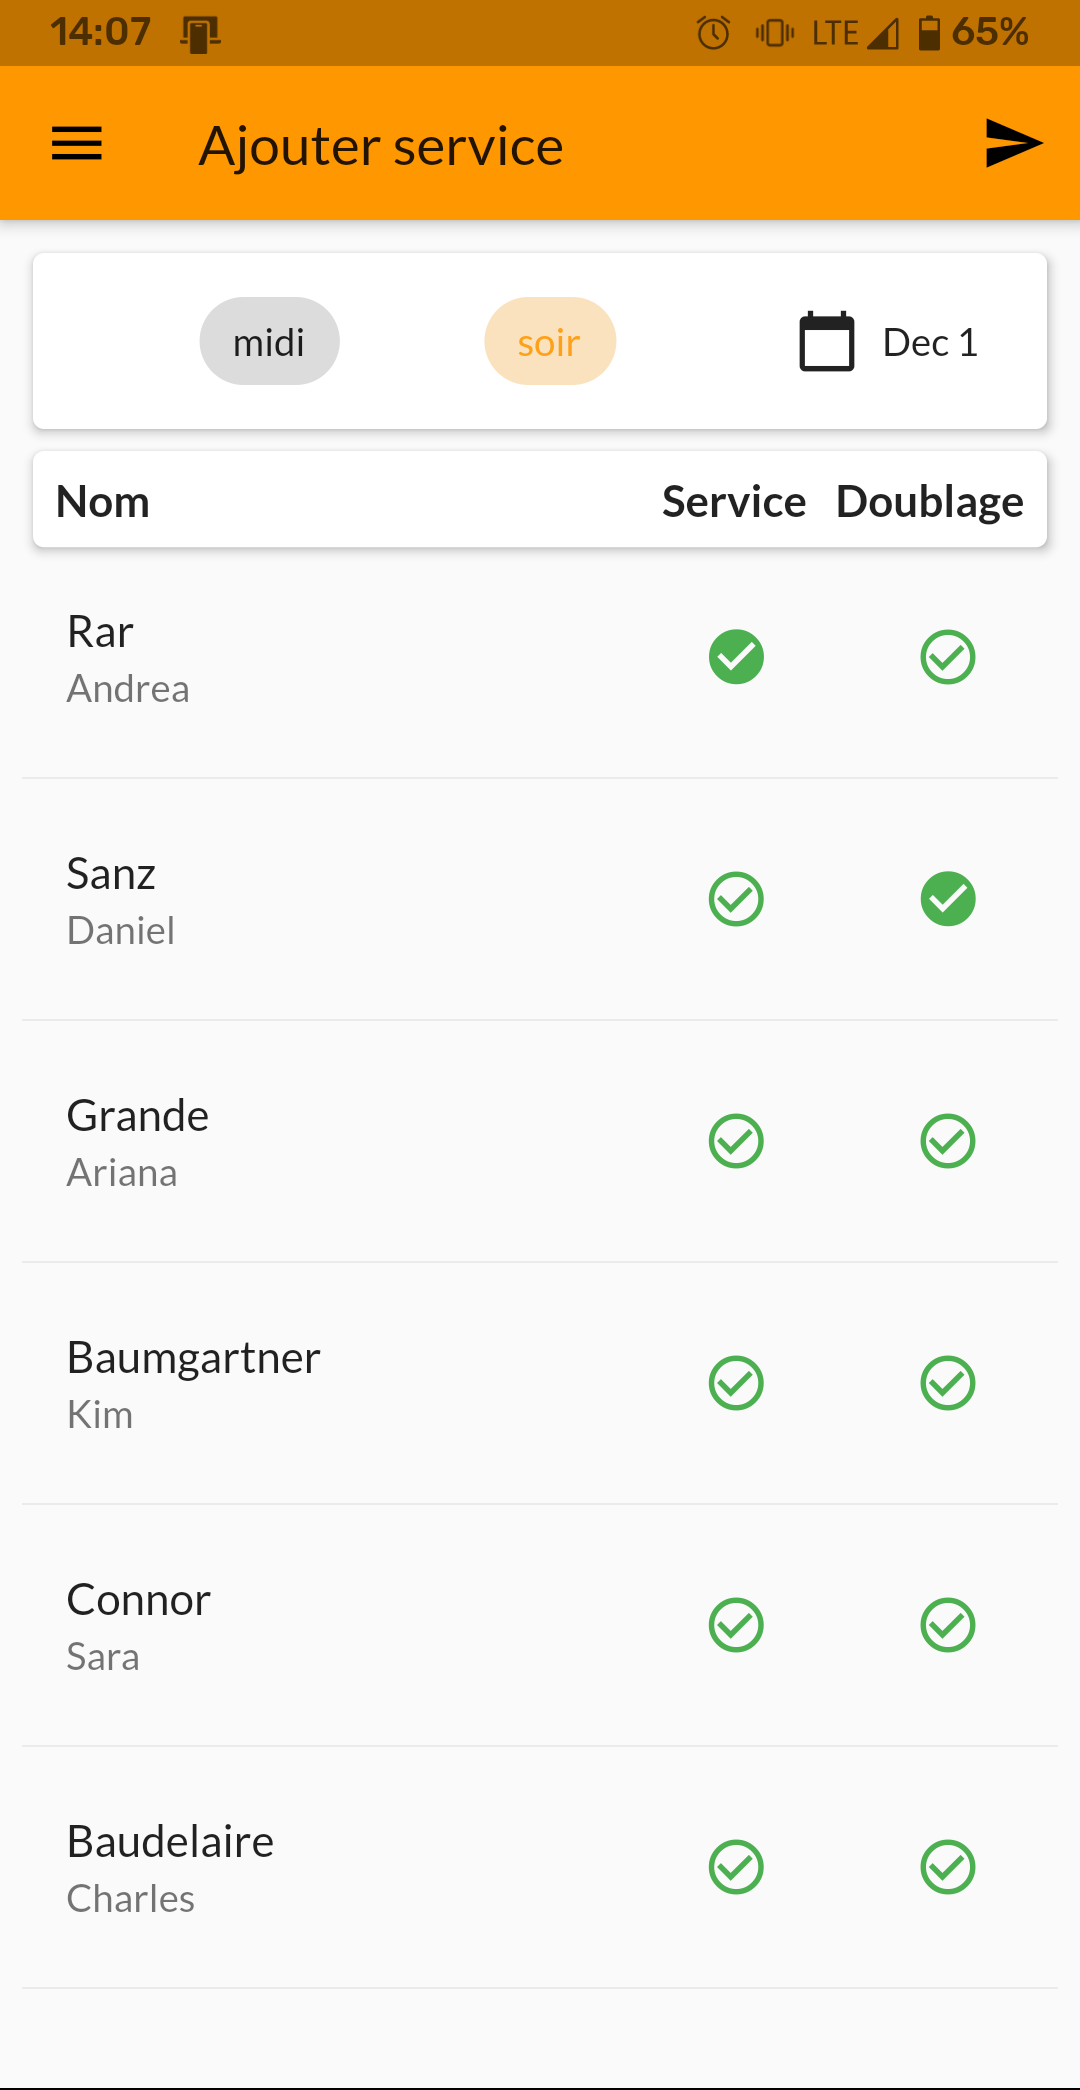
\includegraphics[width=0.6\linewidth]{screenshots/scenario_05/ajout_service_c.png}
            \caption{choix du personnel et type}
            \label{fig:ajout_service_c}
        \end{subfigure}
        \begin{subfigure}{.45\textwidth}
            \centering
            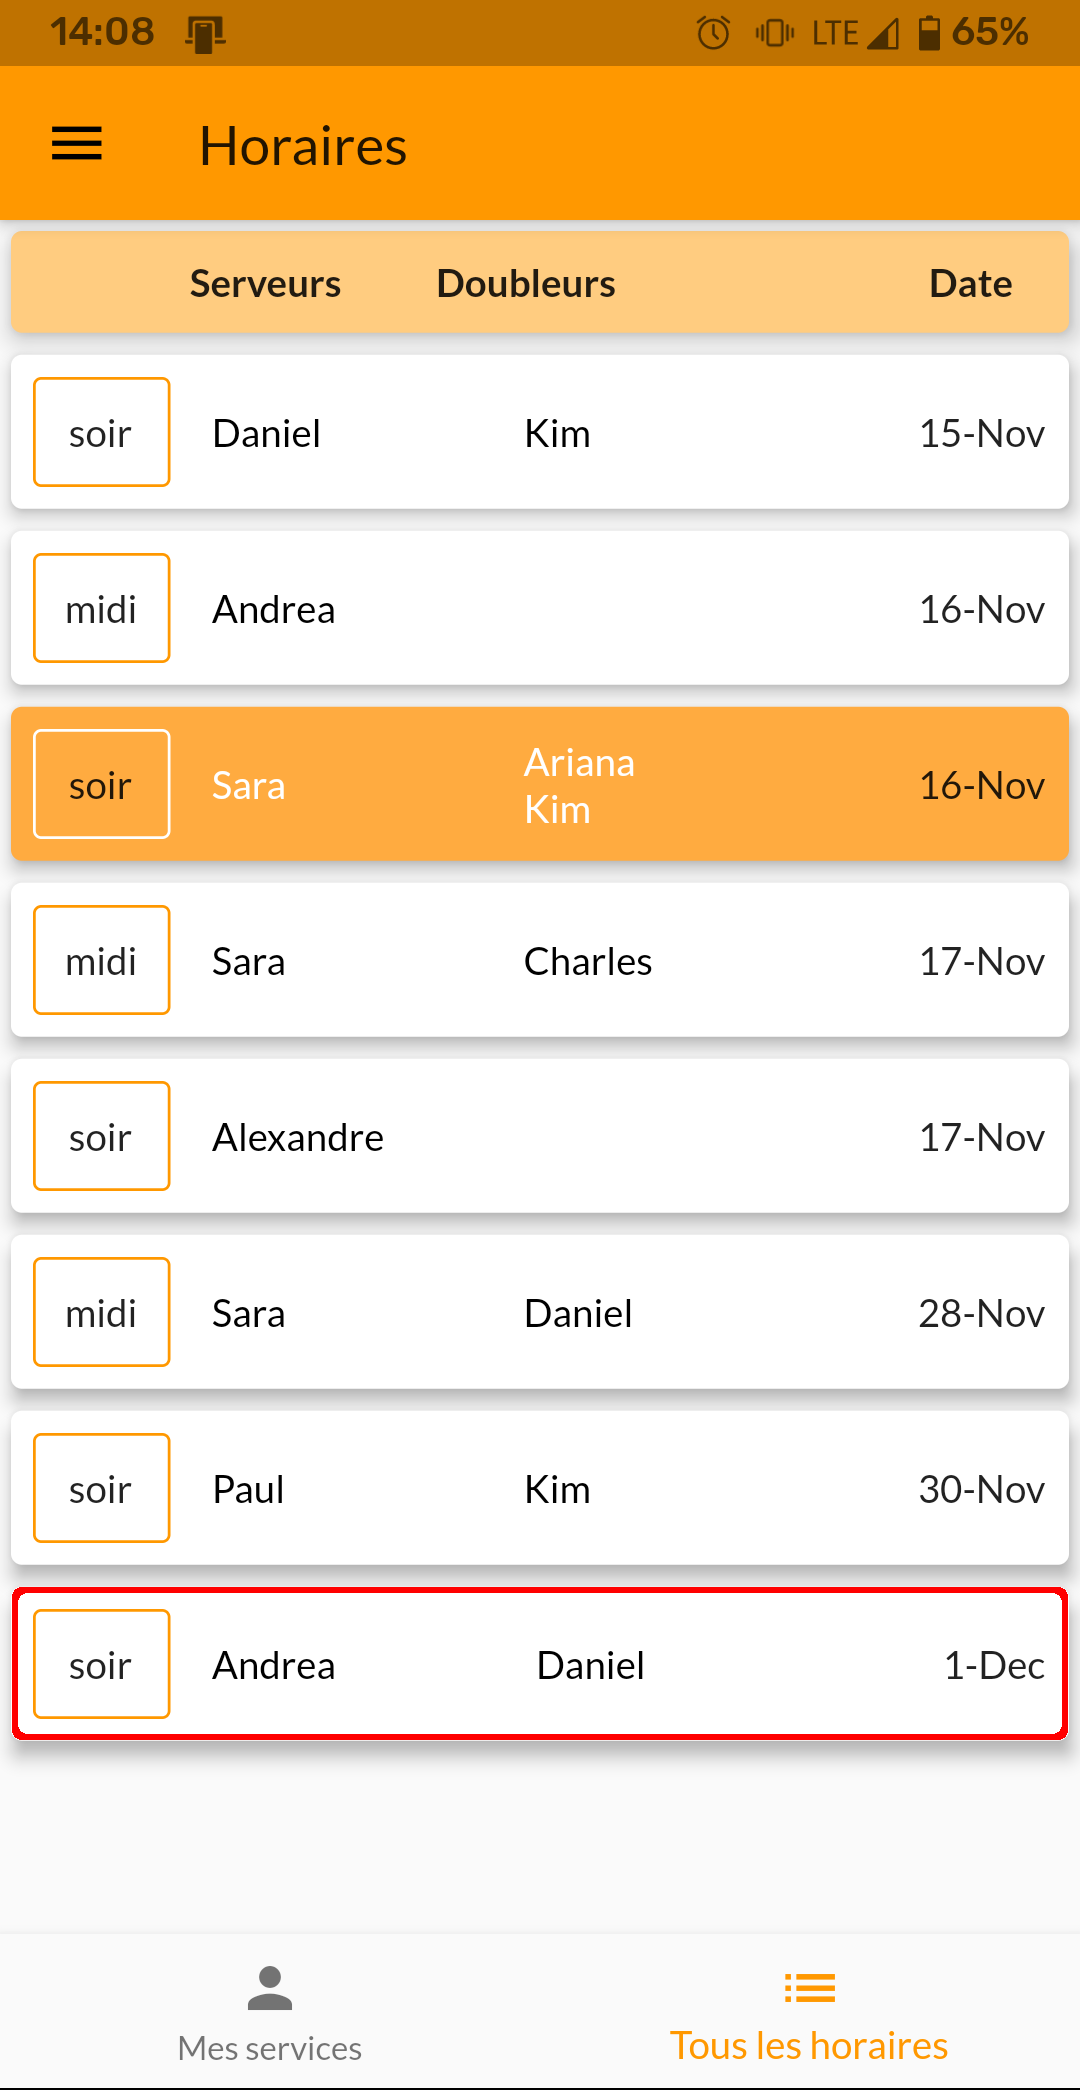
\includegraphics[width=0.6\linewidth]{screenshots/scenario_05/ajout_service_done.png}
            \caption{nouveau service créé}
            \label{fig:ajout_service_done}
        \end{subfigure}
        \caption{scénario V - b}
        \label{fig:scen05b}
    \end{figure}
\end{center}
\newpage
\section[Ajouter un serveur - Scénario VI]{Scénario VI}
    \subsection*{Ajouter un serveur}
    Les utilisateurs ayant les privilèges administrateur ont la capacité
    d'ajouter de nouveaux serveurs.

    \begin{figure}[!h]
        \centering
        \begin{subfigure}{.45\textwidth}
            \centering
            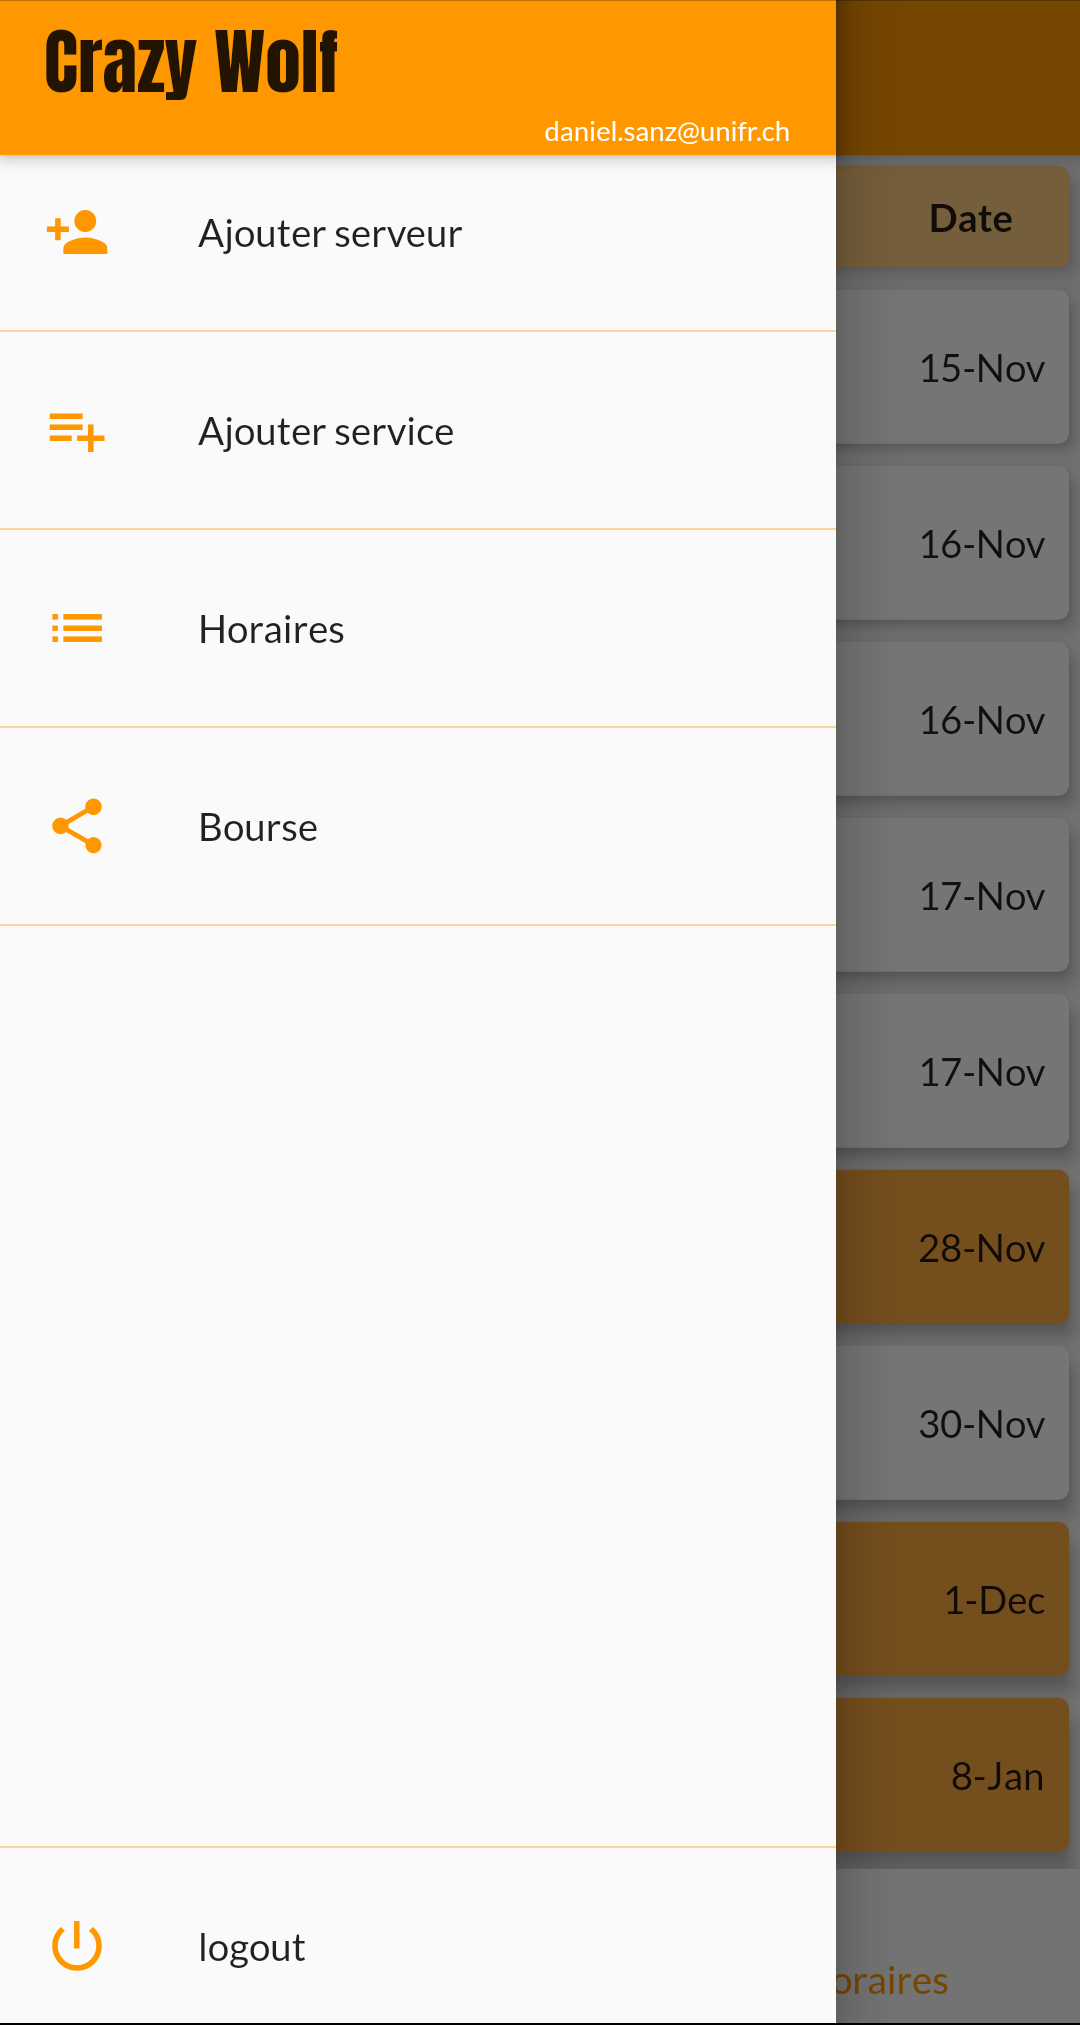
\includegraphics[width=0.6\linewidth]{screenshots/scenario_06/menu_admin.png}
            \caption{menu admin}
            \label{fig:menu_admin}
        \end{subfigure}
        \begin{subfigure}{.45\textwidth}
            \centering
            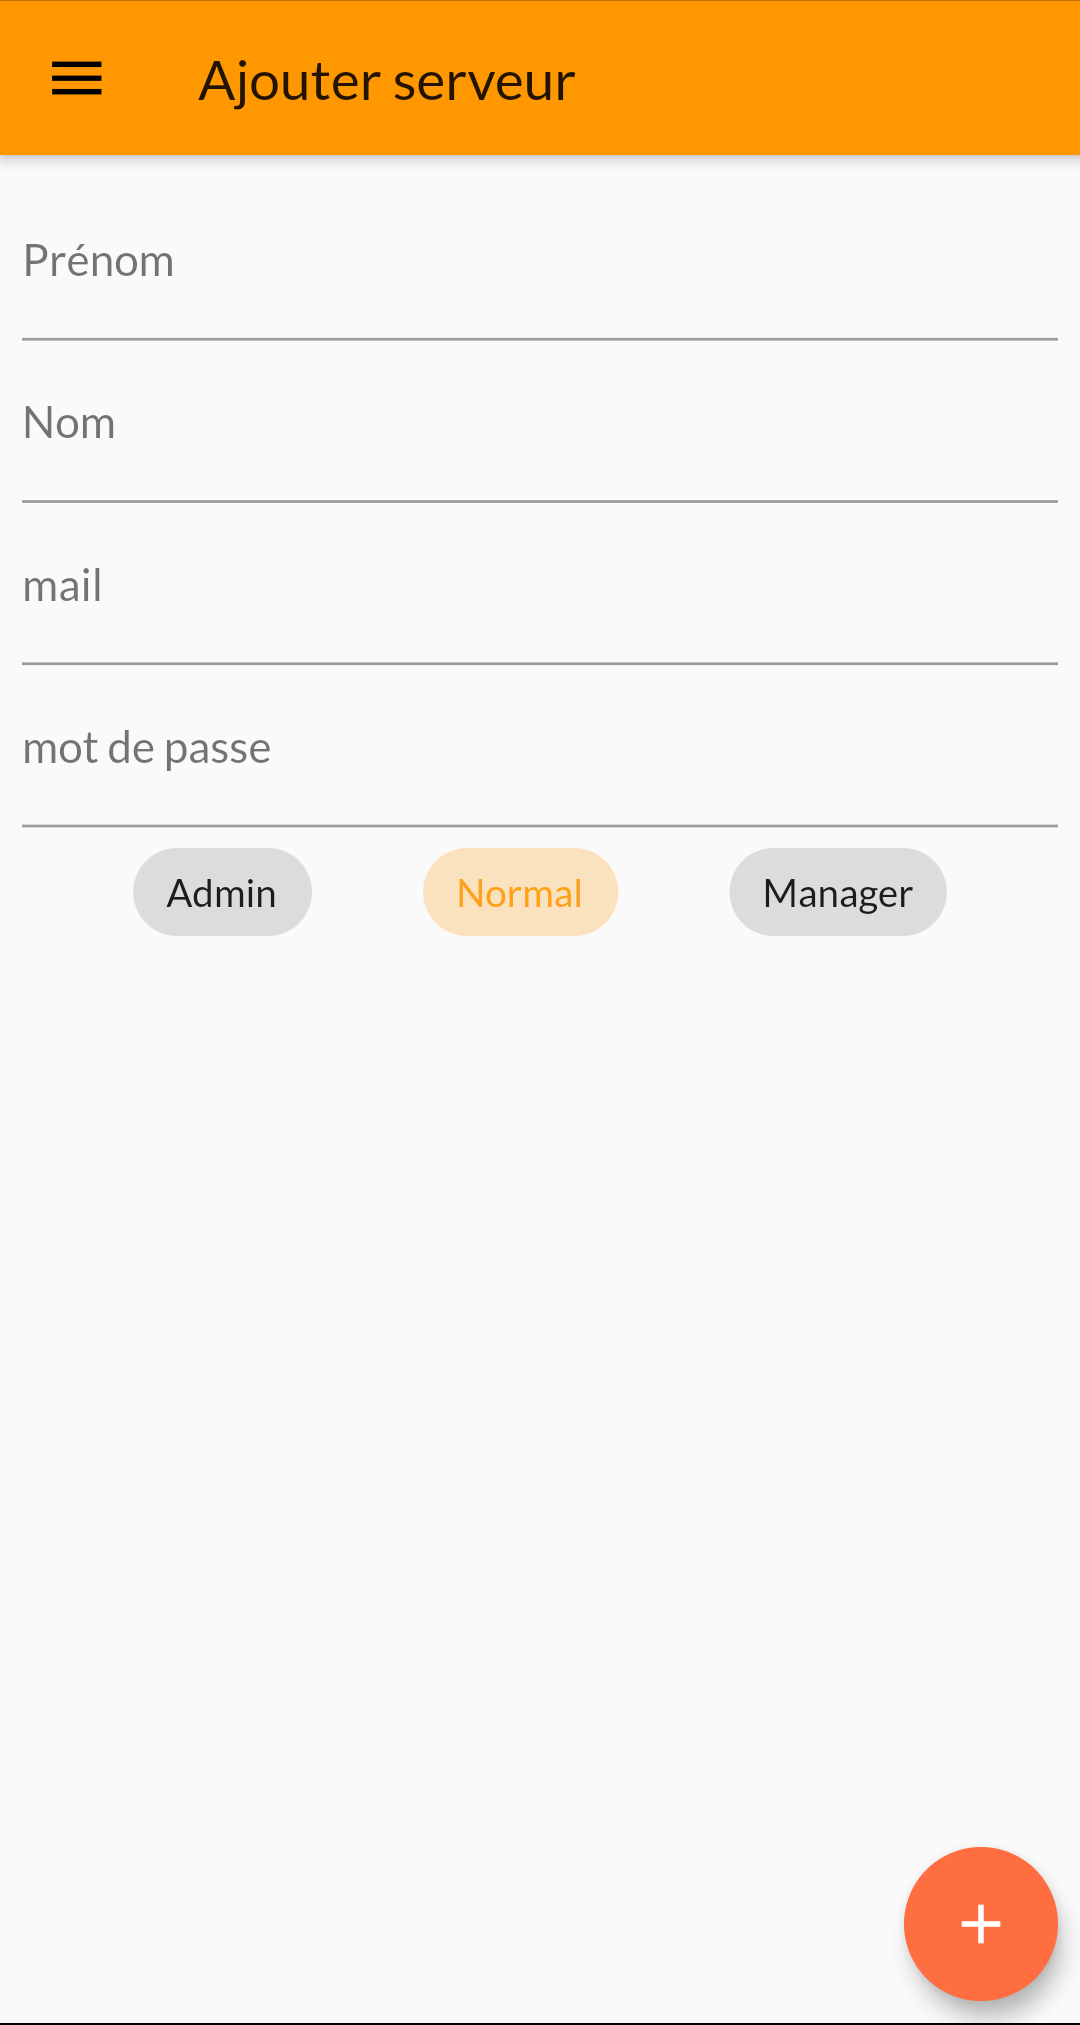
\includegraphics[width=0.6\linewidth]{screenshots/scenario_06/ajout_serveur.png}
            \caption{ajouter serveur}
            \label{fig:ajout_serveur}
        \end{subfigure}
        \caption{scénario VI}
        \label{fig:scen06}
    \end{figure}

    Pour se faire, il doivent après s'être authentifié, naviguer à l'aide 
    du menu latéral \ref{fig:menu_admin} à l'onglet \textit{Ajouter serveur}

    Dans l'onglet \textit{Ajouter serveur} il faut remplir les champs définissant un serveurs. I.e. 
    \smallskip
    \begin{itemize}
        \item Prénom
        \item Nom 
        \item Adresse mail
        \item Mot de passe
        \item Niveau de privilèges: administrateur, normal, manager. 
    \end{itemize}
    \medskip
    Le niveau de privilège le plus courant étant \textit{normal} il est déjà 
    pré-sélectionné.

    Le mot de passe doit être strictement plus long que 6 caractères.

    Utiliser la même adresse mail pour deux serveur différents est interdit. 
    Cependant, deux serveurs peuvent théoriquement avoir le même prénom et le même nom de 
    famille.

    Un fois tous les champs remplis, l'administrateur peut ajouter le serveur
    dans le système en appuyant sur le bouton \textit{+} dans le coin inférieur
    gauche de l'écran \textit{Ajouter serveur} \ref{fig:ajout_serveur}

    Ce sont les indetifiants nécéssaires pour s'authentifier dans l'écran \ref{fig:login}.
    \section[Doublages - Scénario VII]{Scénario VII}
        \subsection*{Doublages}
        Ici on va voir comment un administrateur ou un manager peut demander
        du personnel supplémentaire pour un service. Ces personnes supplémentaires sont dites 
        doubleurs et font un doublage.

        La démarche est similaire à celle d'un échange.

        \begin{figure}[!h]
            \centering
            \begin{subfigure}{.3\textwidth}
                \centering
                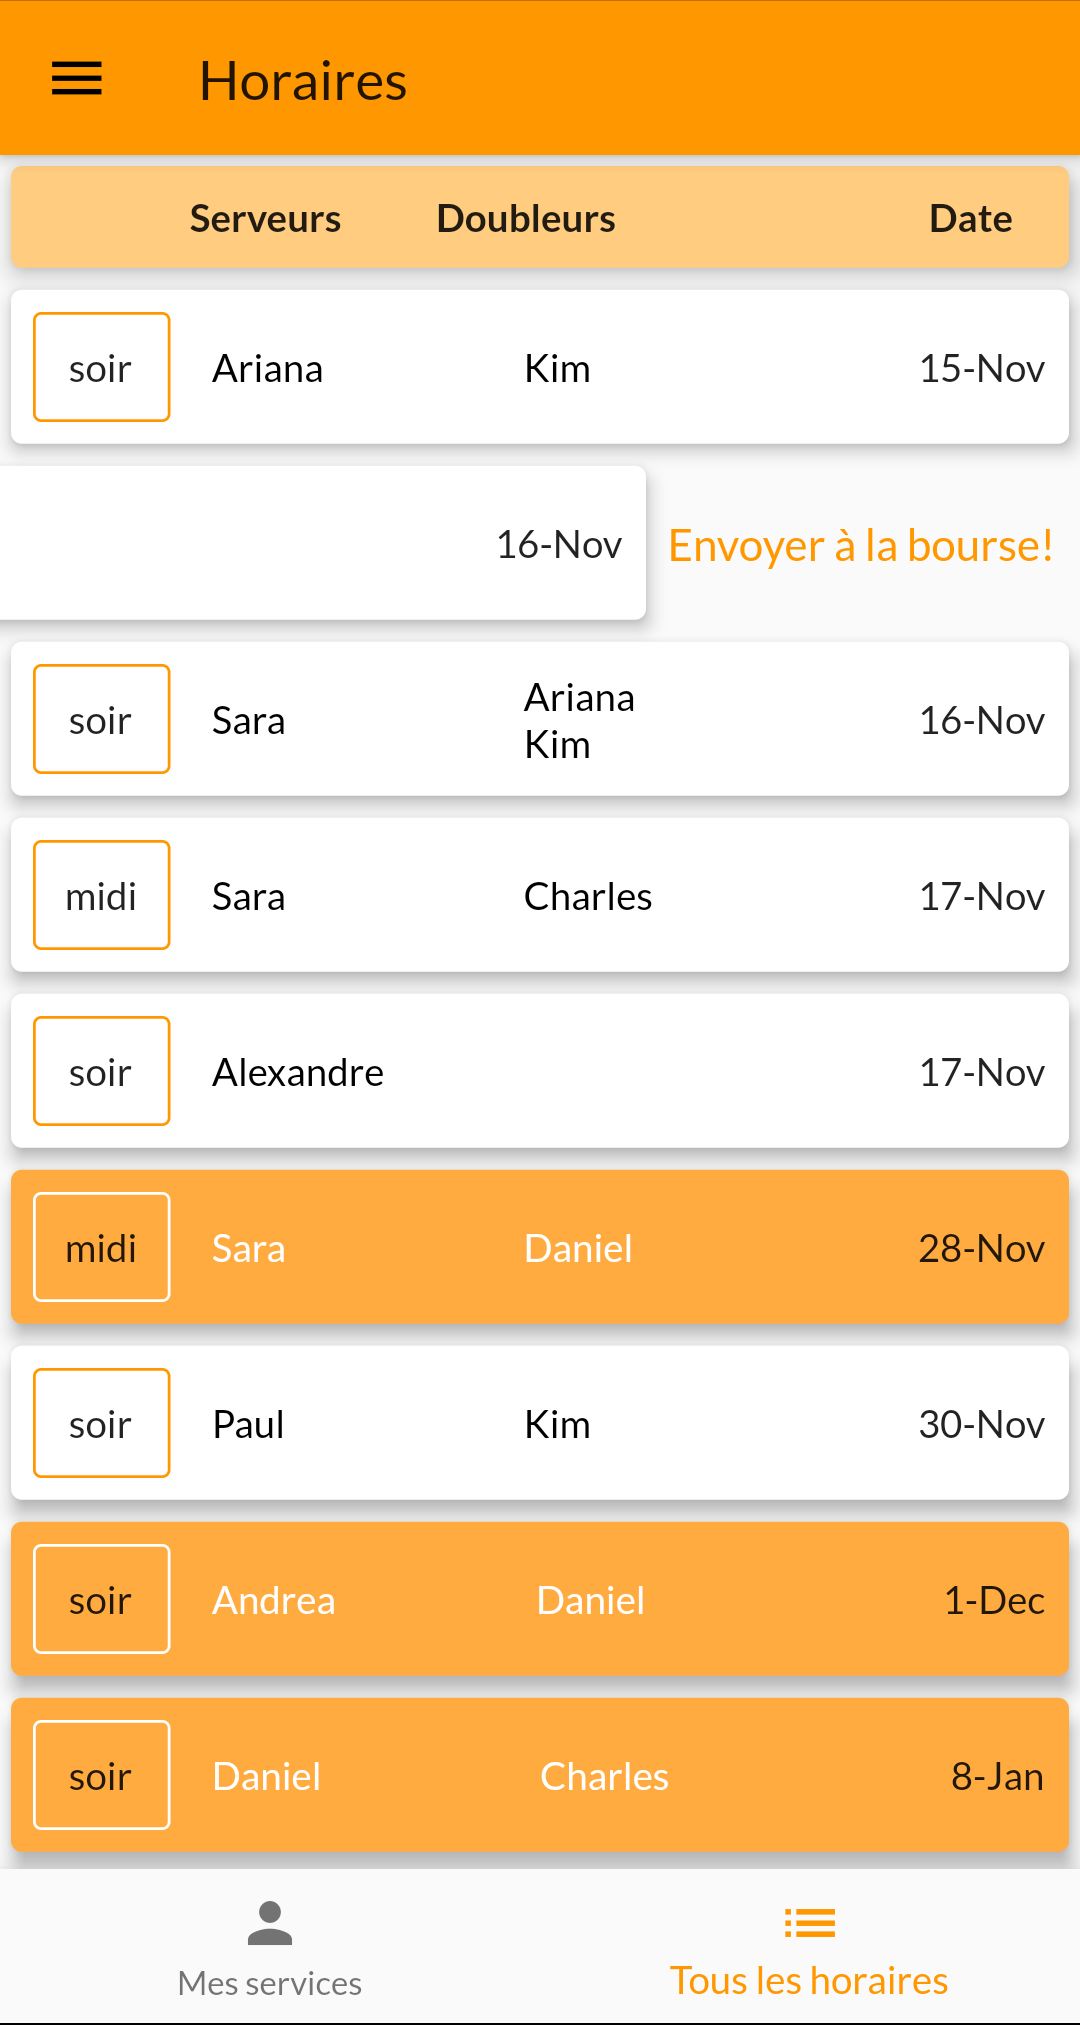
\includegraphics[width=0.9\linewidth]{screenshots/scenario_07/horaire_doublage.png}
                \caption{demande doublage}
                \label{fig:ask_doublage}
            \end{subfigure}
            \begin{subfigure}{.3\textwidth}
                \centering
                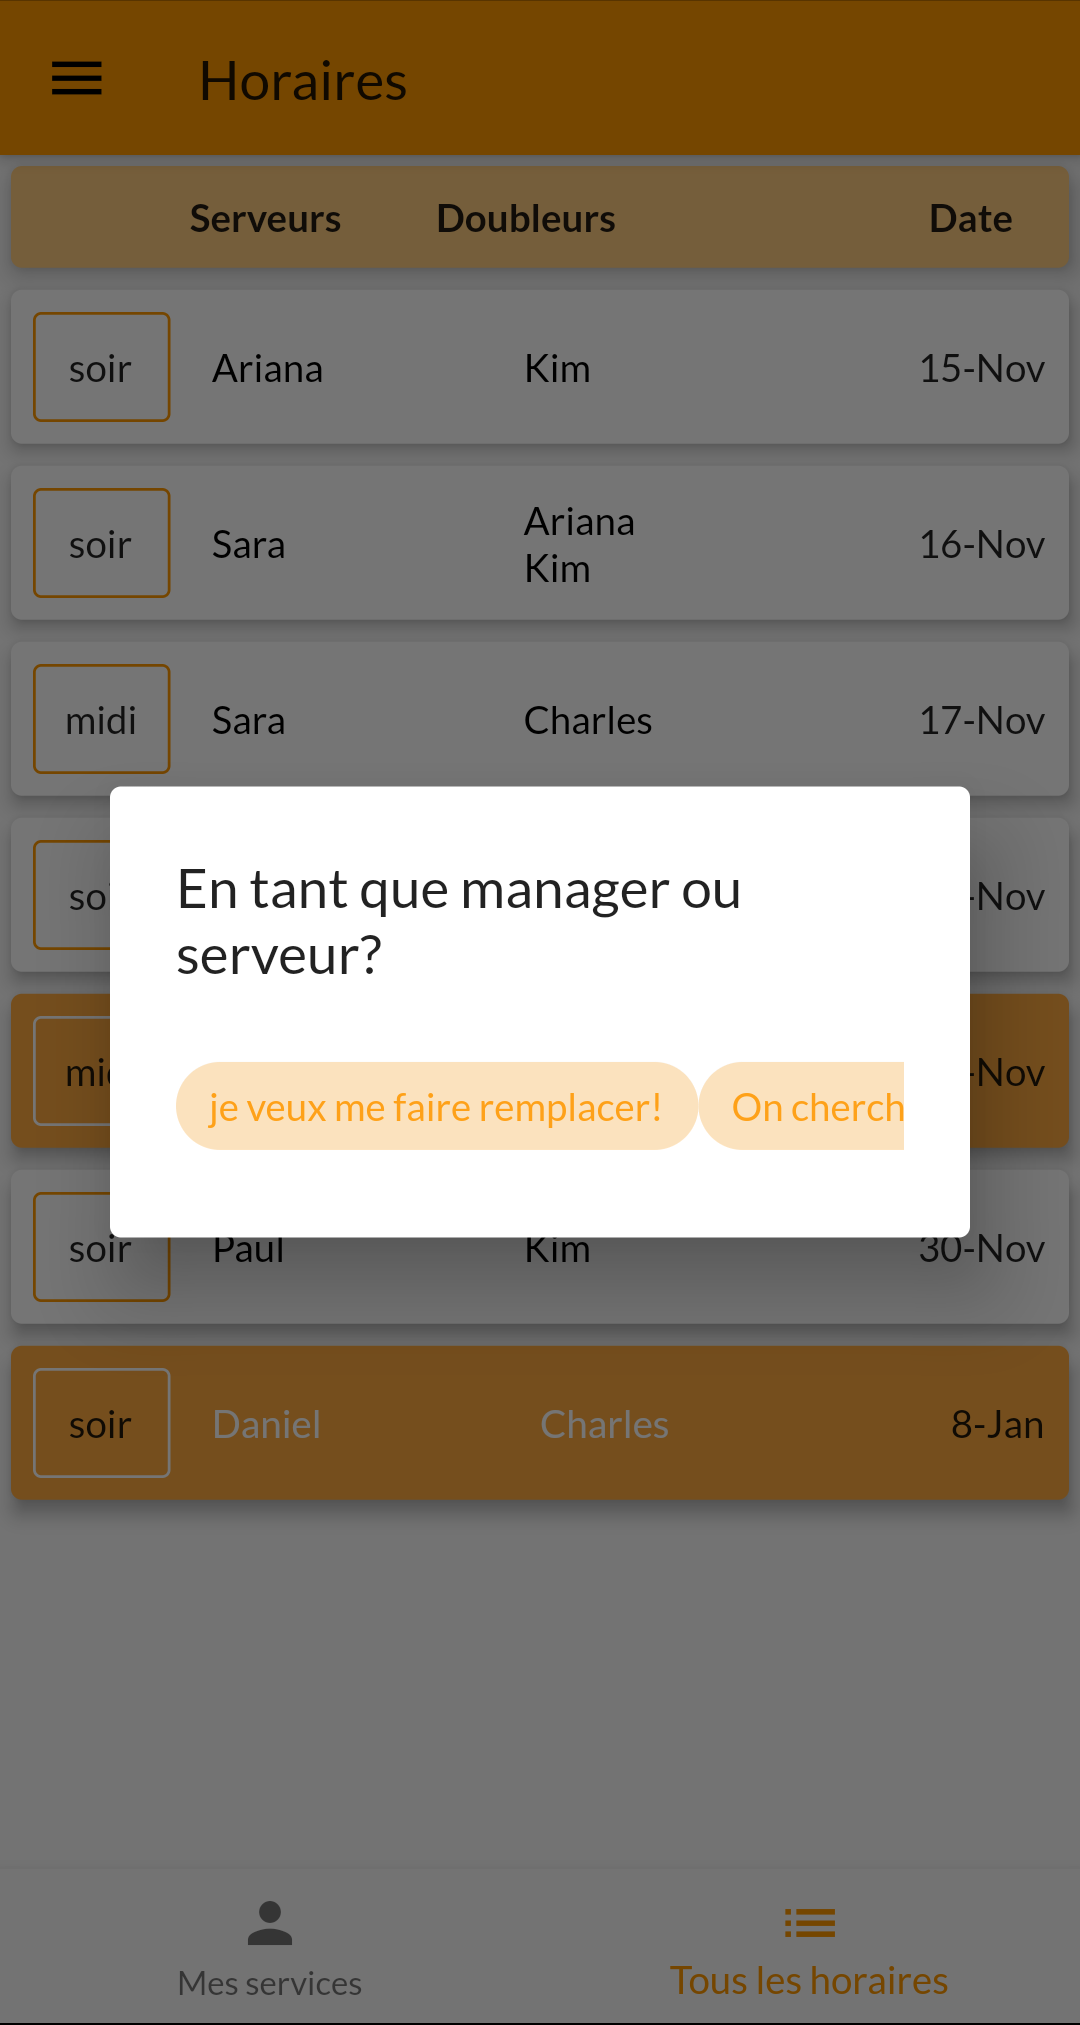
\includegraphics[width=0.9\linewidth]{screenshots/scenario_07/doublage_ou_remplacement.png}
                \caption{remplacement ou doublage}
                \label{fig:ask_doublage2}
            \end{subfigure}
            \begin{subfigure}{.3\textwidth}
                \centering
                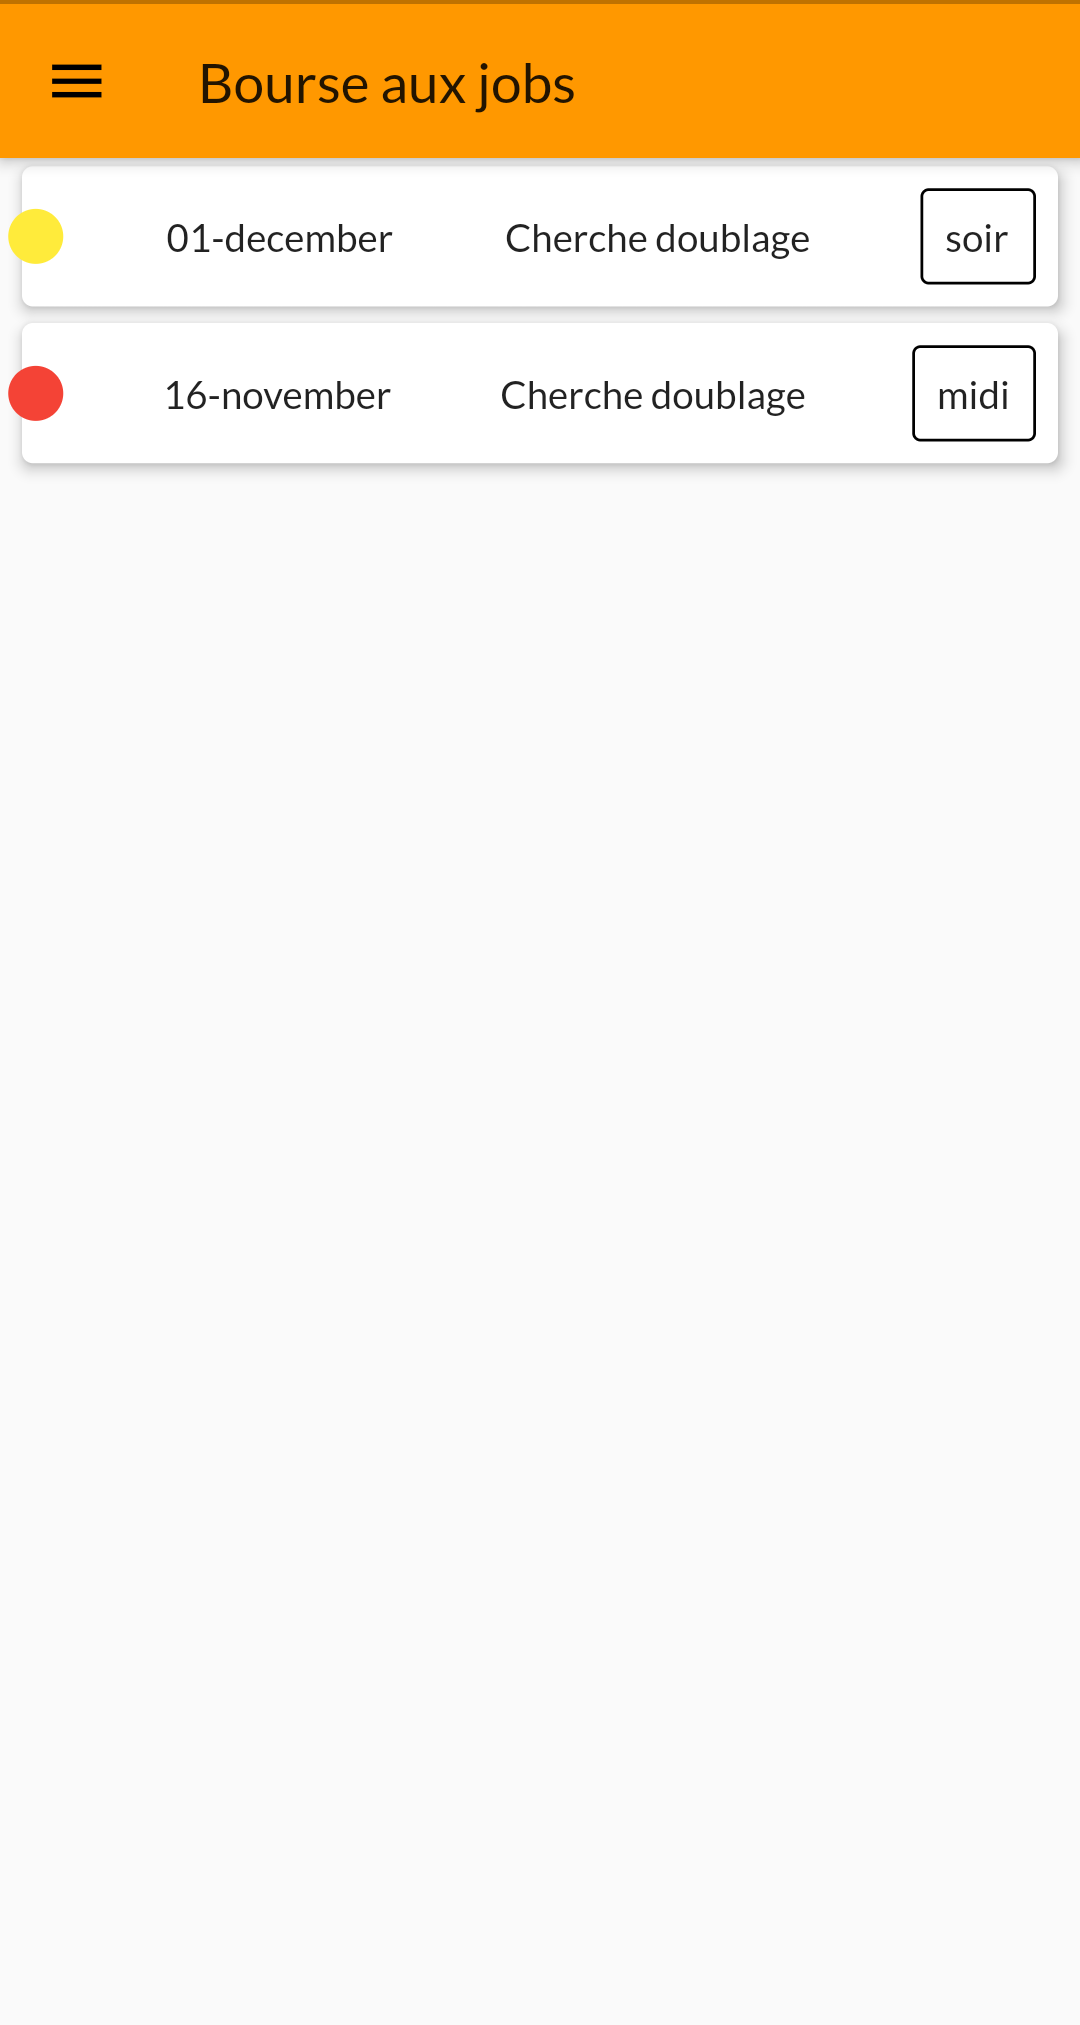
\includegraphics[width=0.9\linewidth]{screenshots/scenario_07/bourse_doublage.png}
                \caption{bourse doublage}
                \label{fig:bourse_doublage}
            \end{subfigure}
            \caption{scénario VII}
            \label{fig:scen07}
        \end{figure}

        Dans un premier temps un utilisateur avec privilèges fait glisser un service 
        sur la gauche \ref{fig:ask_doublage}. Deux options sont possibles suivant si l'utilisateur travaille dans ce
        service ou pas.
        \smallskip
        \begin{itemize}
            \item S'il y travaille alors un popup apparaît \ref{fig:ask_doublage2} pour demander si c'est bien une demande de doublage ou bien se faire remplacer
            \item S'il n'y travaille pas alors la demande de doublage est directement envoyée en bourse.
        \end{itemize}
        \medskip
        Dans cet exemple, deux services sont mis en bourse. 
        Un où l'administrateur n'y travaille pas \ref{fig:ask_doublage}. Comme pour les échange, le degré d'urgence \ref{fig:urgence} est demandé. On peut voir le service du 16 novembre en bourse. 
        Et l'autre où l'administrateur travaille et où il choisit \ref{fig:ask_doublage2} qu'il cherche un doublage.

        À la différence du scénario III \ref{fig:scen03}, la condition pour pouvoir
        accepter des postulants n'est plus d'être l'utilisater ayant mis le service en bourse
        mais d'avoir un niveau de privilèges supérieur à \textit{normal}.
        
        



